\documentclass[onecolumn]{aastex62}
\usepackage{times}
\usepackage{epsfig}
\usepackage{amsmath, amsthm, amssymb}
\usepackage{color}
\usepackage{microtype}
\usepackage{float}
\usepackage{stfloats}
\usepackage{natbib}
\usepackage{verbatim}
%\usepackage{placeins}
\graphicspath{{./figures/}}
\usepackage{wrapfig}
\hypersetup{backref,breaklinks,colorlinks,citecolor=blue}
\usepackage[all]{hypcap}
\usepackage{definitions}
\usepackage{subfiles}

\usepackage{placeins}

\bibliographystyle{apj}

\newcommand{\subdate}{\today}
\newcommand{\shortauth}{Barker et al.}
\newcommand{\slugcom}{Draft - \today}
\newcommand{\TVD}{\textnormal{\tiny\textsc{Tvd}}}
\newcommand{\TCI}{\textnormal{\tiny\textsc{TCI}}}

%\newcommand{\slugcom}{Submitted to ApJL on \subdate}
%\slugcomment{\slugcom}


\lefthead{\sc \footnotesize \slugcom \hfill \shortauth}
\righthead{\sc \footnotesize \slugcom \hfill \shortauth}
%}

\bibliographystyle{aasjournal}
\received{\today}
\shorttitle{Discontinuous Galerkin methods with a nuclear EOS}

\begin{document}

\title{\thornado-hydro: Generalizing discontinuous galerkin methods for a nuclear
equation of state for supernova hydrodynamics}
\author{Brandon Barker}
\affiliation{Department of Physics and Astronomy, University of Tennessee Knoxville, TN 37996}

\author{Eirik Endeve}
\affiliation{Department of Physics and Astronomy, University of Tennessee Knoxville, TN 37996}
\affiliation{Computer Science and Mathematics Division, Oak Ridge National Laboratory, TN 37831}
\affiliation{Joint Institute for Computational Sciences, Oak Ridge National Laboratory, TN 37831}

\author{Anthony Mezzacappa}
\affiliation{Department of Physics and Astronomy, University of Tennessee Knoxville, TN 37996}
\affiliation{Joint Institute for Computational Sciences, Oak Ridge National Laboratory, TN 37831}


\begin{abstract}
A problem of high importance in computational astrophysics is obtaining accurate
solutions to the Euler equations of hydrodynamics. We are interested in solving
the Euler equations in the context of core collapse supernovae.
The toolkit for high-order neutrino-radiation hydrodynamics (\thornado)
is being developed for CCSN simulations and related problems utilizing a spatial discretization
based on the discontinuous Galerkin (DG) method.
The Euler equations form a hyperbolic set of partial differential equations.
In the quasi-linear form, the system can be represented
as a set of independent advection equations that can be limited separately.
This use of characteristic variables also increases the efficiency of the slope
limiting process. However, the addition of the nuclear equation of state equation
to the Euler equations makes the decomposition nontrivial.
We introduce the framework for the characteristic decomposition of the Euler equations
with the inclusion of the nuclear EOS terms and
present results from some initial tests. The results confirm that performing limiting
on the characteristic variables provides better numerical solutions and is
suited to applications in CCSN simulations.
\end{abstract}

\keywords{supernovae: general -- hydrodynamics -- equation of state -- methods: numerical -- discontinuous Galerkin}


\section{Introduction}
\label{sec:Intro}
\todo{Fill in introduction. Contextualize the work.}
The core collapse supernovae (CCSNe) explosion mechanism is fundamentally three-dimensional
in nature \citep[see e.g.,][]{blondin:2006, muller:2012, oconnor:2018b}. Alongside general
reletavistic gravity, complex nuclear equations of state (EOS), and
neutrino transport, hydrodynamics must be accurately modelled,
creating a very challenging and compelling problem. Hydrodynamic instabilities are critical
in aiding the explosion, with complex phenomena such as turbulence and
convection playing key roles in the CCSN mechanism
\citep{murphy:2011, murphy:2013, couch:2013, couch:2015a, radice:2016, mabanta:2018}.
The accurate and efficient modelling of the supernova hydrodynamics is crucial if the
explosion is to be realistically modelled.
For in-depth reviews of the CCSN mechanism, see \citet{bethe:1990, janka:2007, janka:2012a, janka:2016, burrows:2013, hix:2014, muller:2016, couch:2017}.

\todo{Talk about \thornado, DG methods, Euler Equations, possibly reference other codes that
employ different methods and those methods' drawbacks.}

This paper will be organized as follows: in Section \ref{sec:eulereq} we briefly
describe the Euler equations of gas dynamics. Section \ref{sec:DG} describes our
numerical implementation of the DG method in the one dimensional (1D) case.
Section \ref{sec:results} shows the results of 1D hydrodynamic simulations,
and Section \ref{sec:eigen} presents the eigenvectors used in the eigen-decomposition
of the Euler equations.

\section{Euler Equations of Gas Dynamics in Cartesian Coordinates}
\label{sec:eulereq}
\todo{Use this form of the Euler Equations?}
The non-relativistic Euler equations of gas dynamics
\citep[see, e.g.,][for details]{leveque:2002} in Cartesian coordinates
in the absence of sources with a nuclear matter EOS are given by
the equations of conservation of mass,
\beq
  \partial_{t} \rho + \divergence{} (\rho\,  \mathbf{v}) = 0
  \label{eq:massConservation}
\eeq
conservation of momentum,
\beq
%	\partial_{t}(\rho \mathbf{v}) + \divergence{}(\rho u^2 + p) = 0
  \partial_{t}(\rho\,  \mathbf{v}) + \divergence{}(\rho\,  \mathbf{v} \otimes \mathbf{v} + P\, \mathbf{I}) = 0
  \label{eq:momentumConservation}
\eeq
conservation of energy,
\beq
  \partial_{t} E + \divergence{}\left[(E+P)\, \mathbf{v}\right] = 0
  \label{eq:energyConservation}
\eeq
and conservation of \textcolor{red}{electron density}
\beq
  \partial_{t} D + \divergence{}(D\, \mathbf{v}) = 0
  \label{eq:electronConservation}
\eeq
where $\rho$ represents mass density, $\mathbf{v}$ the fluid velocity vector,
$P$ the fluid pressure, $D=\rho y_e$ where $y_e$ is the electron fraction,
$E=\epsilon \rho +\frac{1}{2}\rho v^2$ the total energy (internal plus kinetic),
$\epsilon$ is the specific internal energy, and $\mathbf{I}$ is the identity tensor.
\eqref{eq:massConservation}-\eqref{eq:electronConservation}. The inclusion of
Equation \eqref{eq:electronConservation} is because we require a nuclear EOS.
These equations are closed by a tabulated EOS where the pressure is given by a function of
density, temperature $T$ and the electron fraction: $P = P(\rho, T, y_e)$.
We may rewrite Equations \eqref{eq:massConservation}-\eqref{eq:electronConservation}
in a more convenient way:

\beq
  \partial_{t}\mathbf{U} + \partial_{x}\mathbf{F}(\mathbf{U}) = 0,
  \label{eq:conservation}
\eeq
where $\mathbf{U} =(\rho,\rho \mathbf{v},E, D)^{T}$ is the vector of conserved quantities
and $\mathbf{F}(\mathbf{U})=(\rho \mathbf{v},\rho u^{2}+p,(E+P)\mathbf{v}, D\mathbf{v})^{T}$
is the flux vector.

\section{Numerical Implementation}
\label{sec:DG}

\todo{Add intro paragraph} \\
\textcolor{red}{Subsections or no?}

\subsection{The Discontinuous Galerkin Methods}
In our solver we have chosen the discontinuous Galerkin (DG) method
for our spatial discretization. In this section we will briefly discuss our
implementation of the DG method, introducing notation and concepts.
For simplicity, we will focus on the one dimensional (1D) case. Recall that
we seek solutions to the Euler equations of hydrodynamics, constituting a
conservation law of the form

\beq
  \partial_{t} \mathbf{U} + \partial_{x} \mathbf{F}(\mathbf{U}) = 0
  \label{eq:ode}
\eeq
Where $\mathbf{U}$ is the evolved state vector and $\mathbf{F}(\mathbf{U})$ is
the flux. In order to solve Equation \eqref{eq:ode} numerically, we divide the computational
domain $D\subset \mathbb{R}$ into a disjoint union $\mathcal{T}$ of open elements
$\bK$ such that $D = \cup_{\bK \in \cT}\bK$. Each element $\bK$ is a box in the
coordinates
\beq
  \bK \in (\xL,x_{R}),
\eeq
We let the approximation space $\mathbb{V}^{k}$ for the DG method
be constructed from the tensor product of one-dimensional
polynomials of degree $k$. Note that functions in $\mathbb{V}^{k}$
can be discontinuous across element interfaces. The DG problem is then to find
$\mathbf{U}_h \in \mathbb{V}^{k}$ which approximates $\mathbf{U}$ in Equation
\eqref{eq:ode}, such that $\forall$ $\phi \in \mathbb{V}^{k}$ and $\bK \in \cT$

\beq
  \partial_{t} \int_{\bK}\mathbf{U}_h\, \phi\, dx +
  \int_{\bK}\partial_{x}\, \mathbf{F(\mathbf{U})}\, \phi\, dx = 0.
\label{eq:semidiscreteDG_almost}
\eeq
Integrating the second term by parts, this becomes
\beq
   \partial_{t} \int_{\bK}\mathbf{U_{h}}\, \phi\, dx +
   \widehat{\mathbf{F}}(\mathbf{U}_h)\, \phi^{-} \big|_{x_{R}}
   + \widehat{\mathbf{F}}(\mathbf{U}_h)\, \phi^{+} \big|_{x_{L}} +
   \int_{\bK}\mathbf{F(\mathbf{U}_h)}\, \partial_{x}\phi\, dx = 0.
\label{eq:semidiscreteDG}
\eeq
In Eq.~\eqref{eq:semidiscreteDG}, $\widehat{\vect{F}}(\vect{U}_{h})$ is a
numerical flux approximating the flux on the boundary of $\bK$.
The numerical flux function is evaluated using values from
both boundaries of an element; i.e.,
\begin{equation}
  \widehat{\vect{F}}(\vect{U}_{h})=\vect{f}(\vect{U}_{h}(x^{-}),\vect{U}_{h}(x^{+})),
\end{equation}
where superscripts $-/+$
indicate that the function is evaluated to the immediate left/right of the
interface. We use the Harten-Lax-van Leer (HLL) flux \citep{harten:1983}
for all the numerical experiments presented in Section \ref{sec:results}.

In each element $K$, we use a nodal representation of the conserved variables
$\mathbf{U}$:

\beq
\begin{split}
  \mathbf{U}(x,t) \approx\, & \mathbf{U}_h (x,t) =
  \sum_{i=1}^{N}\vect{U}_{i}(t)\,\ell_{i}(x),
  \quad\text{where}\quad \\
  & \ell_{i}(\eta)=
  \prod_{\substack{j=1\\j\ne i}}^{N}\f{\eta-\eta_{j}}{\eta_{i}-\eta_{j}}
  \label{eq:conservedNodalExpansion}
\end{split}
\eeq
are Lagrange polynomials defined on $I = \{ \eta : \eta \in (-0.5,0.5) \}$,
and are constructed to interpolate the node set
$S_{N}=\{\eta_{i}\}_{i=1}^{N}\subset I$. The spatial coordinate $x$ and the
reference coordinate $\eta$ are related by the
mapping $x(\eta)=\xL+(0.5+\eta)\,\Delta x$.
Then, for any $\eta_{j}\in S_{N}$, $\ell_{i}(\eta_{j})=\delta_{ij}$,
so that $\vect{U}_{h}(x(\eta_{j}),t)=\vect{U}_{j}(t)$.
First we define the $M$-point quadrature $Q_{M}:C^{0}(I)\to\mathbb{R}$
with abscissas $\hat{S}_{M}=\{\eta_{q}\}_{q=1}^{M}$ and weights
$\{w_{q}\}_{q=1}^{M}$, normalized such that $\sum_{q=1}^{M}w_{q}=1$ in order to
evaluate the integrals in Eq.~\eqref{eq:semidiscreteDG}.
We use the $M$-point Legendre-Gauss quadrature, which is exact for
polynomials of degree $\le 2M-1$.
Then, if $P_{h}(x)$ is such a polynomial, we have
\beq
  \f{1}{\Delta x}\int_{K}P_{h}(x)\,dx=\int_{I}P_{h}(\eta)\,d\eta=\sum_{q=1}^{M}w_{q}\,P_{h}(\eta_{q}).
\eeq

For the sake of efficiency we let $M=N$ and $S_{N}=\hat{S}_{N}$, which is a
spectral-type nodal collocation DG approximation \citep{bassi:2013}.
Inserting Eq.~\eqref{eq:conservedNodalExpansion} into Eq.~\eqref{eq:semidiscreteDG},
letting $\phi(x)=\ell_{k}(x)$, using the quadratures defined above,
we obtain
\begin{align}
  \pd{}{t}\int_{K}\vect{U}_{h}\,\phi\,dx
  &\approx w_{k}\,\pd{}{t}\vect{U}_{k}\,\Delta x
  \label{eq:timeDerivativeTerm}
\end{align}
for the time derivative piece.
Similarly, the last term on the left-hand side of Eq.~\eqref{eq:semidiscreteDG}
becomes
\beq
  \int_{K}\vect{F}(\vect{U}_{h})\,\pderiv{\phi}{x}\,dx
  \approx \sum_{q=1}^{N}w_{q}\,\vect{F}(\vect{U}_{q})\,\pderiv{\ell_{k}}{\eta}(\eta_{q}).
  \label{eq:volumeTerm}
\eeq
Now we may combine Eqs.~\eqref{eq:timeDerivativeTerm}-\eqref{eq:volumeTerm} in
Eq.~\eqref{eq:semidiscreteDG} resulting in the semi-discrete form
\beq
  \deriv{\vect{U}_{k}}{t}
   =-\f{1}{w_{k}\Delta x}
  \Big\{
  \Big[\,
    \widehat{\vect{F}}\ell_{k}\big|_{x_{H}}
     -\widehat{\vect{F}}\ell_{k}\big|_{\xL}
  \,\Big]
   -\sum_{q=1}^{N}w_{q}\,\vect{F}(\vect{U}_{q})\,\pderiv{\ell_{k}}{\eta}(\eta_{q})
  \Big\}.
  \label{eq:semidiscreteDiscretized}
\eeq
We now have a system of ordinary
differential equations (ODEs), which may be evolved in time with an ODE solver.
In Section~\ref{sec:results} we use the third-order strong
stability-preserving Runge-Kutta (SSP-RK3) method \citep{shu:1988}.

\subsection{Slope Limiting}
\label{sec:Limiting}
A common feature of high-order numerical PDEs is unphysical oscillations in the solutions,
particularly near discontinuities.
It is therfore of great interest in the DG algorithm to implement slope limiting
of the polynomial $\mathbf{U}_h$. We use the total variation diminishing (TVD)
slope limiter \citep[see, e.g.,][]{cockburn:1998} in conjunction with the
troubled cell indicator discussed in \citet{fu:2017} to prevent excessive limiting
by flagging elements where limiting is needed. To do this, we need to reduce under- and
overshootings of the higher-order solution at cell boundaries compared to
the cell averages of neighbor cells. Recall from Eq.~\eqref{eq:conservedNodalExpansion}
that in each cell our solution is expressed as

\beq
\mathbf{U}_h (x,t) =
\sum_{l=1}^{N}c_{l}(t)\,P_{l}(x)
\eeq

\noindent where we have chosen to expand in the Legendre polynomials. We compare
the weight $c_{1}$, which is proportional to the first derivative of the
solution in the cell, to the neighboring cell averages by the following

\beq
  \widetilde{c}_{1} = \text{minmod}(c_{1},
    \beta_{\TVD}(c_{0}^{+} - c_{0}), \beta_{\TVD}(c_{0} - c_{0}^{-}))
  \label{eq:limiting}
\eeq

\noindent where $\widetilde{c}_{1}$ is the limited weight. Here, we used the minmod
function defined as

\beq
  \text{minmod}(a_{1}, a_{2}, a_{3}) =
   \begin{cases}
      s\,\, \text{min}\{\abs{a_{1}}, \abs{a_{2}}, \abs{a_{3}}\} &
        s = \text{sign}(a_{1})= \text{sign}(a_{2})= \text{sign}(a_{3}) \\
      0 & \text{otherwise.}
   \end{cases}
\label{eq:minmod}
\eeq

Limiting is applied to each component of the vector of conserved quantities
separately and is generally referred to as `Componentwise limiting.`
The parameter $\beta_{\TVD}$ takes values in the closed interval $\left[1,2\right]$
and scales the strength of the limiting. A minimal $\beta_{\TVD}$ corresponds with
the total variation diminishing scheme \textcolor{red}{reference?} but is more
dissipative than the maximal $\beta_{\TVD}$ case, which is more flexible but allows for more oscillations.
Increasing $\beta_{\TVD}$ puts more weight on the neighboring cell averages,
making the minmod function more likely to set $ \widetilde{c}_{1} = c_{1}$.

In order to determine where slope limiting is necessary, we use the
troubled cell indicator (TCI) \citep{fu:2017} to prevent excessive limiting:\footnote{Would this notation be altered for 1D?}

\begin{equation}
  I_{\bK}(G) = \f{\sum_{j}|G_{\bK}-G_{\bK}^{(j)}|}{\max_{j}|G_{\bK^{(j)}}^{(j)}|},
  \label{eq:tci}
\end{equation}

\noindent where $G\in\vect{G}\subseteq\vect{U}$ and $\vect{G}$ consists of the
first and final elements of $\vect{U}$. Here, the sum in the numerator and the
max in the denominator are taken over the neighboring elements sharing a
boundary with target element $\bK$, $G_{\bK}$ is the cell average in $\bK$,
$G_{\bK}^{(j)}$ is the cell average
computed by extrapolating the polynomial representation from the neighboring
element $\bK^{(j)}$ into $\bK$, and $G_{\bK^{(j)}}^{(j)}$
is the cell average native to neighbor element $\bK^{(j)}$. An element is flagged
for limiting if, for any $G\in\vect{G}$, $I_{\bK}(G)>C_{\TCI}$, where
$C_{\TCI}$ is a defined threshold.

\subsection{Time Integration}
\label{sec:TimeInt}
The general $s$-stage Runge-Kutta time stepping algorithm, including
the limiting process, can be summarized as in \citet{cockburn:2001}:
\begin{itemize}
  \item[1.] Set $\bar{\vect{U}}^{(0)} = \bar{\vect{U}}^{n}$,
  \item[2.] For $i=1,\ldots,s$ compute:
  \begin{equation}
  \small  \bar{\vect{U}}^{(i)}
    = \Big\{\Lambda^{\TVD}\Big\{\sum_{j=0}^{i-1}\alpha_{ij}\,\bar{\vect{U}}^{(j)}+\beta_{ij}\,\Delta t\,\bar{\vect{F}}\big(\bar{\vect{U}}^{(j)}\big)\Big\}\Big\},
    \label{eq:rkStages}
  \end{equation}
  \item[3.] Set $\bar{\vect{U}}^{n+1}=\bar{\vect{U}}^{(s)}$.
\end{itemize}
Above, the TVD limiter limiter preventing unphysical
states is denoted by the operators $\Lambda^{\TVD}\{\}$. The SSP-RK3 coefficients $\alpha_{ij}$
and $\beta_{ij}$ may be found in Table~2.1 in \citet{cockburn:2001}. For each step
in Eq.~\eqref{eq:rkStages}, the TVD limiter is applied to elements flagged
by the troubled cell indicator.\textcolor{red}{Discuss timestepping conditions?}

\subsection{Characteristic Decomposition}
\label{sec:characteristicDecomp}
Experience has shown that the slope limiting described in the previous section
is more effecient when performed on the so-called `characteristic variables`
as opposed to the conserved variables $\mathbf{U}_h$
\citep[see, e.g.,][for a description]{cockburn:1998}. We begin by
rewriting Eq.~\eqref{eq:conservation} in the quasi-linear form as follows
\beq
  \pderiv{\mathbf{U}}{t}
  + \pderiv{\mathbf{U}}{\mathbf{x}} \pderiv{\mathbf{F(\mathbf{U})}}{\mathbf{U}}
  = 0.
  \label{eq:charEq}
\eeq
Because the Euler equations for a systemer of hyperblic
partial differential equations \citep[see, e.g.,][]{leveque:1992}, we can decompose the
Jacobian of the flux vector as

\beq
  \pderiv{\mathbf{F(\mathbf{U})}}{\mathbf{U}} =
  \mathcal{R} \Lambda \mathcal{R}^{-1},
\eeq
where the columns of $\mathcal{R}$ contain the right eigenvectors of the Jacobian,
the rows of $\mathcal{R}^{-1}$ contain the left eigenvectors, and
$\Lambda$ is a diagonal matrix containing the eigenvalues of the Jacobian.
At this point, we will introduce the characteristic variable
$\mathbf{w} = \mathcal{R}^{-1}\mathbf{U}$. Multiplying both sides of Equation
\eqref{eq:charEq} by $\mathcal{R}^{-1}$, we are able to linearize the system of equations to
a system of advection equations

\beq
  \pderiv{\mathbf{w}}{t} +
  \Lambda \pderiv{\mathbf{w}}{x}
  = 0.
\eeq
Solutions to these advection equations are far simpler to obtain than the
previous equations. Limiting may then be applied to dampen oscillations in the
solutions for the characteristic variables $\mathbf{w}$, which are then
transformed back to the solution of the conserved variables $\mathbf{U}$
\citep[see e.g.,][for a description]{cockburn:1998, schaal:2015a}. While this
process of characteristic limiting has been done for the ideal EOS
\citep[][]{cockburn:1998}, we want
to extend to the nuclear matter EOS case.


\section{Derivation of Jacobian and Eigenvalues for the 3D Nuclear Case}
\label{sec:eigen}

We assume that $P = P(\tau, \epsilon, n)$, where $\tau = \frac{1}{\rho}$.
Let the vector of conserved variables be $\textbf{U} = \{\rho, m_1, m_2, m_3, E, D\}$,
where $m_i = \rho v_i$ and $D = \rho y_{e}$.
The flux vector is $\textbf{F}(\textbf{U}) =
\{m_{1}, m_{1}^{2}\tau + P, m_{1}m_{2}\tau, m_{1}m_{3}\tau,
(E+P)m_{1}\tau, Dm_{1}\tau\}$. The Jacobian of the flux vector is given by


%\begin{table*}[ht!]

\begin{align}
  \centering
	\pderiv{\mathbf{F}(\mathbf{U})}{\mathbf{U}}
	= \left[
		\begin{array}{cccccc}
			0 & 1 & 0 & 0 & 0 & 0 \\
			-v_{1}^{2} -P_{\tau}\tau^{2} - P_{\epsilon}\tau(\epsilon - \frac{v^{2}}{2}) & v_{1}(2-P_{\epsilon}\tau)  & -P_{\epsilon}v_{2}\tau & -P_{\epsilon}v_{3}\tau  & P_{\epsilon}\tau  & P_{D_{e}} \\
			-v_{1}v_{2} & v_2 & v_1 & 0 & 0 & 0 \\
			-v_{1}v_{3} & v_{3} & 0 & v_{1} & 0 & 0 \\
			v_{1}(-H - P_{\tau}\tau^{2} -P_{\epsilon}\tau(\epsilon - \frac{v^{2}}{2})) & H - P_{\epsilon}v_{1}^{2}\tau  & -P_{\epsilon}v_{1}v_{2}\tau & -P_{\epsilon}v_{1}v_{3}\tau  & v_{1}(1+P_{\epsilon}\tau) & v_{1} P_{D_{e}} \\
			-v_{1} y_{e} & y_{e} & 0 & 0 & 0 & v_{1} \\
		\end{array}
    \right]
\end{align}
%\caption{}
%\end{table*}


\noindent Where $H=(E+P)\tau$ is the specific enthalpy and $P_{x} = \partial_{x}P$\footnote{Maybe define these elsewhere to show what's constant}. The eigenvalues of this Jacobian are given by

\begin{align}
\Lambda =
\begin{bmatrix}
  v_{1} - c_{s} & 0 & 0& 0& 0& 0 \\
  0 & v_{1} & 0 & 0 & 0 & 0      \\
  0 & 0 & v_{1} & 0 & 0 & 0      \\
  0 & 0 & 0 & v_{1} & 0 & 0      \\
  0 & 0 & 0 & 0 & v_{1} & 0      \\
  0 & 0 & 0 & 0 & 0 & v_{1} + c_{s}
\end{bmatrix}
\end{align}
where $c_{s} = \sqrt{\Gamma P \tau}$, for
$\Gamma = \frac{\tau (P P_{\epsilon} - P_{\tau}) + P_{D_e} y_{e} \tau^{-1}}{P}$, is
the local sound speed. In the ideal EOS regime this reduces to the sound speeds given \citet{colella:1985}.
The right eigenvectors are then given by
\begin{align*}
  \mathcal{R}_{1} =
  \left[
  \begin{array}{cccccc}
   1 & 0 & 1 & 1 & 0 & 1 \\
   v_{1}-c & 0 & v_{1} & v_{1} & 0 & c+v_{1} \\
   v_{2} & 1 & 0 & 0 & 0 & v_{2} \\
   v_{3} & 0 & 0 & 0 & 1 & v_{3} \\
   h-c v_{1} & v_{2} & \beta & 0 & v_{3} & h+c v_{1} \\
   y_{e}  & 0 & 0 & \frac{\tau  \chi }{2 P_{D_{e}}} & 0 & y_{e}  \\
  \end{array}
  \right]
\end{align*}
where the follow definitions have been used:
$h_{n} = \frac{c^2}{P_{\epsilon}\tau} + k $, $k = \frac{-y_{e} P_{D_{e}} \tau^{-1}
+ P_{\epsilon} (\frac{1}{2}v^2 + \epsilon) + P_{\tau}\tau}{P_{\epsilon}}$,
$\delta_{1} = v_{1}^{2}-v_{2}^{2}-v_{3}^{2}$,
$\chi = P_{\epsilon} ( \delta_{1} + 2\epsilon) + 2P_{\tau}\tau$, and
$\beta = \frac{1}{2} (\delta_{1}+2 \epsilon +\frac{2 P_{\tau} \tau }{P_{\epsilon}})$.
The matrix of left eigenvectors is given by

\begin{align*}
  \mathcal{R}_{1}^{-1} = \frac{1}{c^2}
  \left[
  \begin{array}{cccccc}
   \frac{1}{4} (2 c  v_{1}+\omega ) & \frac{1}{2} (-c- \phi_{1} ) & -\frac{1}{2} \phi_{2}
    & -\frac{1}{2} \phi_{3}  & \frac{P_{\epsilon} \tau }{2} & \frac{P_{D_{e}}}{2}
     \\
   -\frac{v_{2} \omega }{2} & \phi_{1} v_{2}  & c^2+\phi_{2} v_{2}  &
     \phi_{3} v_{2}  & -\phi_{2}  & -P_{D_{e}} v_{2}
     \\
   \frac{2 \chi  c^2+\alpha  \omega \tau^{-1} }{2 \chi } & -\frac{\phi_{1} \alpha  }{\chi \tau } &
     -\frac{\phi_{2} \alpha  }{\chi \tau } & -\frac{\phi_{3} \alpha }{\chi \tau } &
     \frac{P_{\epsilon} \alpha }{\chi } & \frac{P_{D_{e}} \left(\alpha -2 c^2\right)}{\tau \chi }
      \\
   -\frac{y_{e} P_{D_{e}} \omega }{\chi \tau } & \frac{2 y_{e} P_{D_{e}} \phi_{1} }{\chi \tau } & \frac{2 y_{e} P_{D_{e}}
     \phi_{2} }{\chi \tau} & \frac{2 y_{e} P_{D_{e}} \phi_{3} }{\chi \tau} & -\frac{2 y_{e}
     P_{D_{e}} P_{\epsilon} }{\chi } & \frac{2 P_{D_{e}} \left(c^2-y_{e} P_{D_{e}} \right)}{\tau  \chi }
      \\
   -\frac{v_{3} \omega }{2} & \phi_{1} v_{3}  & \phi_{2} v_{3}   &
     c^2+\phi_{3} v_{3}  & -\phi_{3}  & -P_{D_{e}} v_{3}
      \\
   \frac{1}{4} (\omega -2 c  v_{1}) & \frac{1}{2} (c-\phi_{1} ) & -\frac{1}{2} \phi_{2}
       & -\frac{1}{2} \phi_{3}  & \frac{P_{\epsilon} \tau }{2} & \frac{P_{D_{e}}}{2}
     \\
  \end{array}
  \right]
\end{align*}
where $\phi_{i} = P_{\epsilon}\,\tau\, v_{i}$,
$\omega = \tau\, (P_{\epsilon}\,(v^2 - 2\epsilon) - 2\,P_{\tau}\,\tau)$, and
$\alpha = 2 y_{e} P_{D_{e}} - \tau \chi$.


The left and right eigenvectors presented here are similar in form to those
presented in \citet{schaal:2015}, but are considerably messier due to the
restriction of a nuclear EOS.

\section{Preliminary Numerical Results}
\label{sec:results}
In this section we present preliminary numerical results obtained with the DG
method implemented in \thornado\, leveraging use of the characteristic
decomposition. Unless otherwise noted, we use the SFHo EOS of
nuclear matter \citep{steiner:2013} now commonly used in high-fidelity CCSN simulations.
These tests serve to gauge the performance improvement of the
DG characteristic decomposition implementation on a set of benchmarks as an initial
assessment of its suitability for future CCSN simulations.

\subsection{Sod Shock Tube}
We present the classic 1D Sod shock tube Riemann problem \citep{sod:1978} in
Cartesian coordinates. The computational domain is D = [-5,5] km
with a discontinuity initially located at $x = 0$ km separating the left and right states

\begin{align}
  \mathbf{U}_{L} &= (10^{12}~\text{g~cm}^{-3}, 0\,, 3.712*10^{32}~\text{ergs~cm}^{-3}, 0.4*10^{12})^T\,\,\, \\
  \mathbf{U}_{R} &= (1.25*10^{11}~\text{g~cm}^{-3}, 0\, , 3.015*10^{31}~\text{ergs~cm}^{-3}, 0.375*10^{11})^T.
\end{align}
\footnote{\textbf{Fix e in the state vectors}}
\noindent The test is run until $t = 0.025$ms with 100 elements
using $C_{\TCI} = 0.2$ and $\beta_{\TVD} = 2.0$. Results are plotted in
Figure~\ref{fig:SodSedovOptimal}. Using the characteristic limiting described
above, the DG method captures the features of the solution without introducing
noticeable oscillations in the solutions near the discontinuities. In Figure~\ref{fig:shock}
we plot elements in the $xt$-plane flagged by the troubled cell indicator for
limiting.

\begin{figure}[h!]
  \centering
  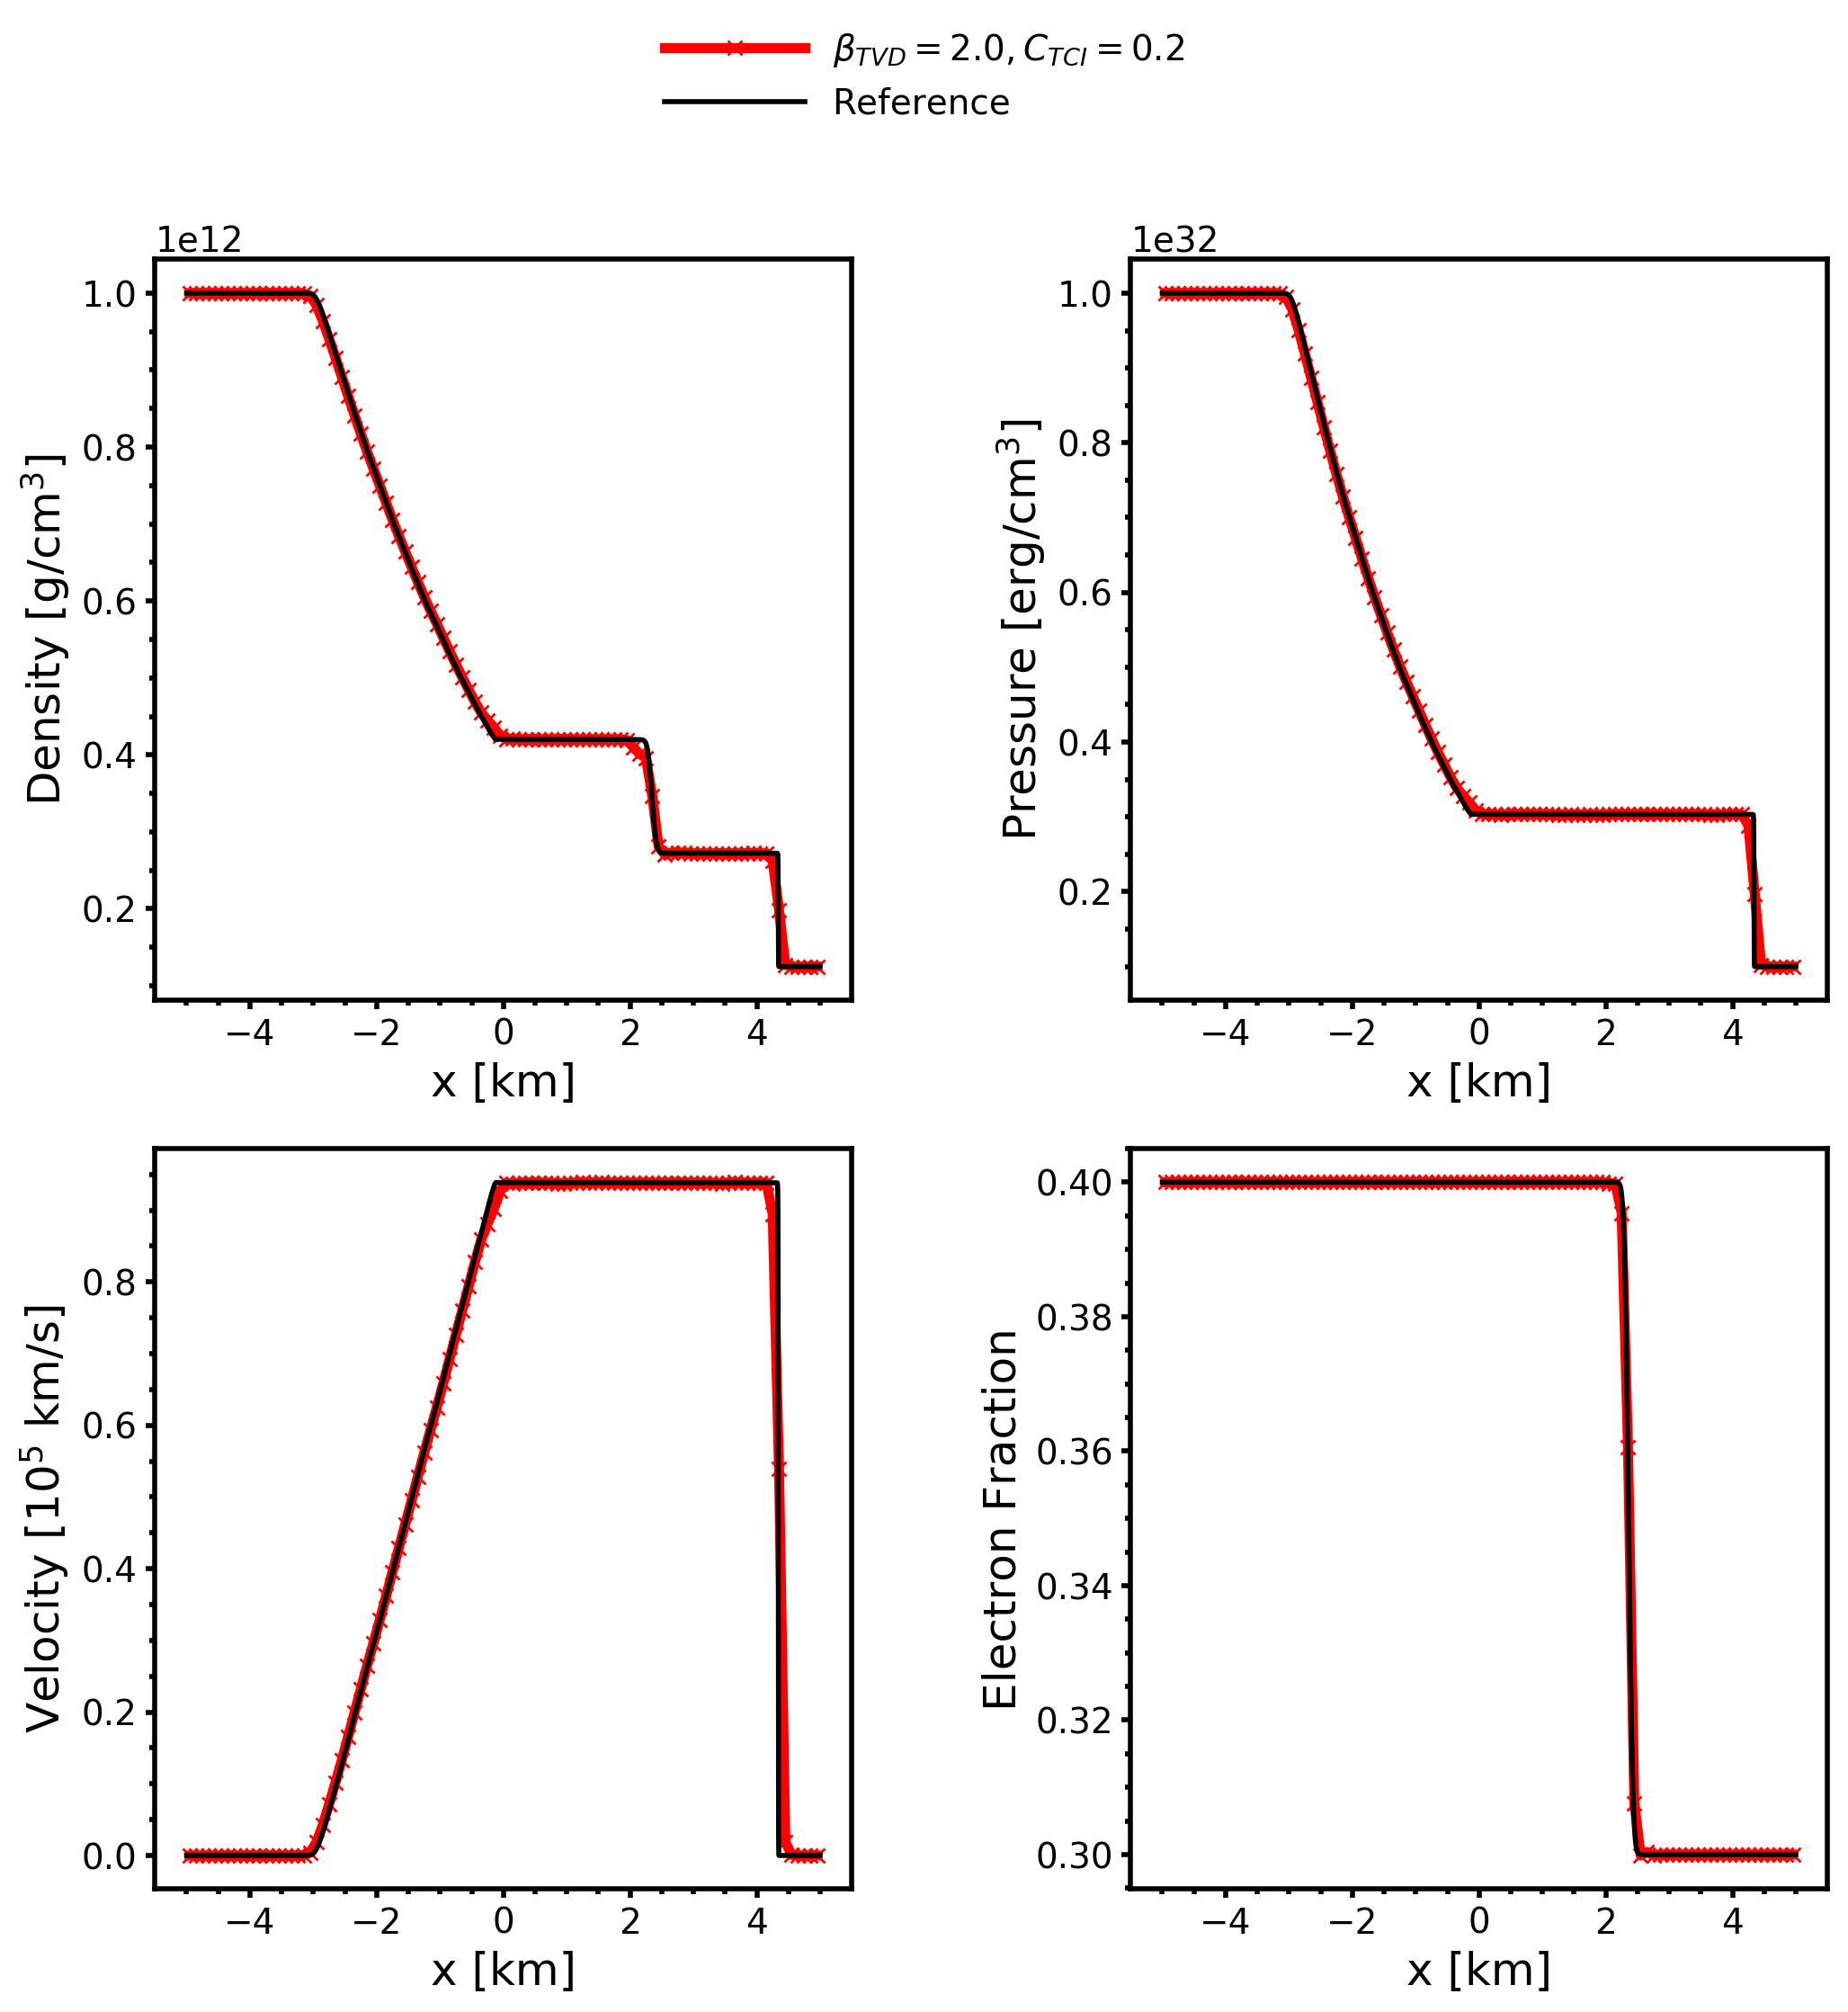
\includegraphics[width=32pc,height=30pc]{optimal.png}
  \centering
  \caption{\label{fig:SodSedovOptimal} Numerical solution of Sod's problem using
    100 elements compared with a reference solution using 10000 elements.}
\end{figure}
%\clearpage
\begin{wrapfigure}{L}{2.8in}
  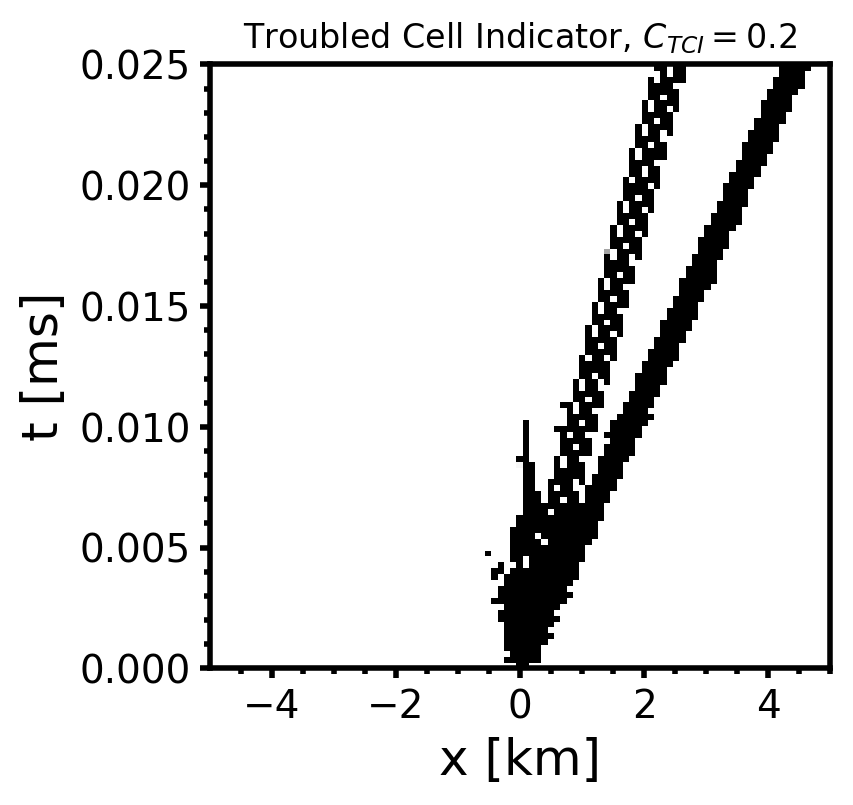
\includegraphics[width=18pc]{optimal_shock.png}
  \caption{$xt$-plane of elements flagged for limiting by the troubled cell indicator.}
  \label{fig:shock}
\end{wrapfigure}

\subsection{Optimal Limiting Parameters}
\label{sec:param}
In order to determine the optimal limiting parameters $C_{\TCI}$ and $\beta_{\TVD}$,
we performed a suite of sixteen simulations of Sod's problem with various
limiting parameters with $\beta_{\TVD}\in\left[1.0,2.0\right]$ and
$C_{\TCI}\in\left[0.0,0.2\right]$. For each $\left(\beta_{\TVD},C_{\TCI}\right)$ pair,
we computed the relative error and total variation \textbf{\textcolor{red}{EQUATIONS}} in density and electron
fraction at $t = 0.025$ms. Results are plotted in Figure~\ref{fig:landscape}.
We find that, as expected, increasing $\beta_{\TVD}$ tends to monotonically
decrease the relative error while (non-monotonically) increasing the total variation due to the
limiter allowing for more oscillations. Increasing $C_{\TCI}$ tends to decrease
the relative error and increase the total variation.
We have selected
$\beta_{\TVD}=1.75$ and $C_{\TCI}=0.1$ to be the optimal parameters providing
the best combination of relative error and total variation reduction. Unless
otherwise noted, all following results will use this combination of limiting
parameters.

\begin{figure}[b]
  \centering
  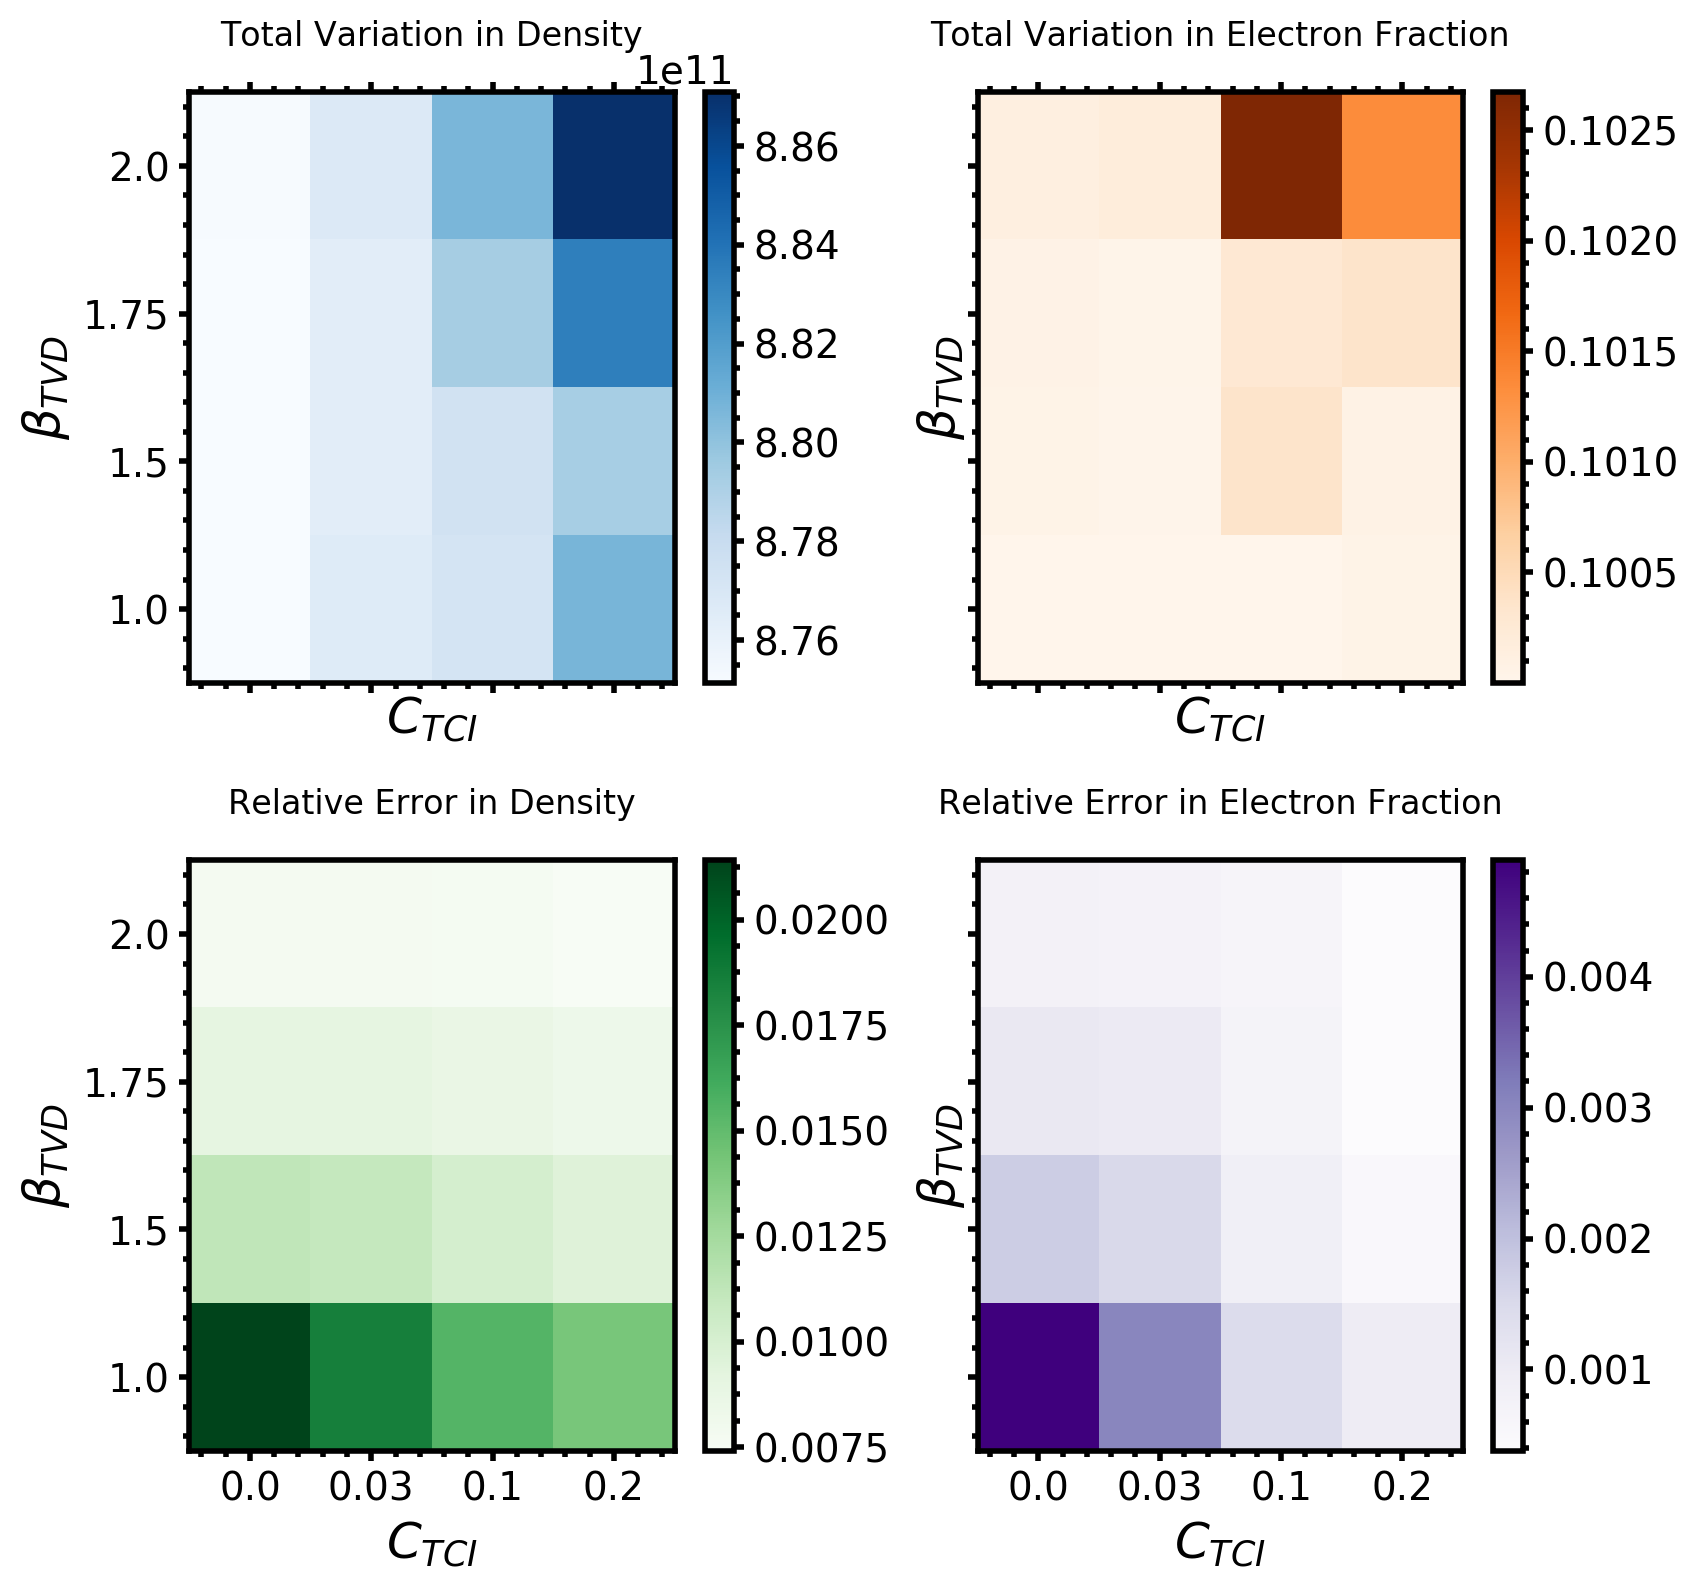
\includegraphics[width=32pc, height=27.5pc]{./figures/error_tv_landscape.png}
  \caption{\label{fig:landscape} Error - total variation landscapes for various
  values of the limiting parameters $C_{TCI}$ and $\beta_{TVD}$.}
\end{figure}

\subsection{Improvement From Componentwise Limiting}
\label{sec:optimal}
The motivation for limiting on the characteristic variables is the potential
improvement from componentwise limiting. In Figure~\ref{fig:SodSedovCW} we plot the
solution at $t = 0.025$ms using 100 elements employing both characteristic
limiting (blue) and componentwise limiting (red) compared to a reference
solution computed with 10000 elements. We observe, for the componentwise limiting,
noticable oscillations in density around the contact discontinuity as well
as less resolved discontinuities. The electron fraction displays very
large oscillations at the left side of the contact discontinuity, up to
$\pm 0.02$ in the cell averaged electron fraction. This makes characteristic
limiting particularly appealing for CCSN simulations where the electron fraction
plays a critical role in the explosion dynamics.

% \begin{figure}[h]
%   \centering
%   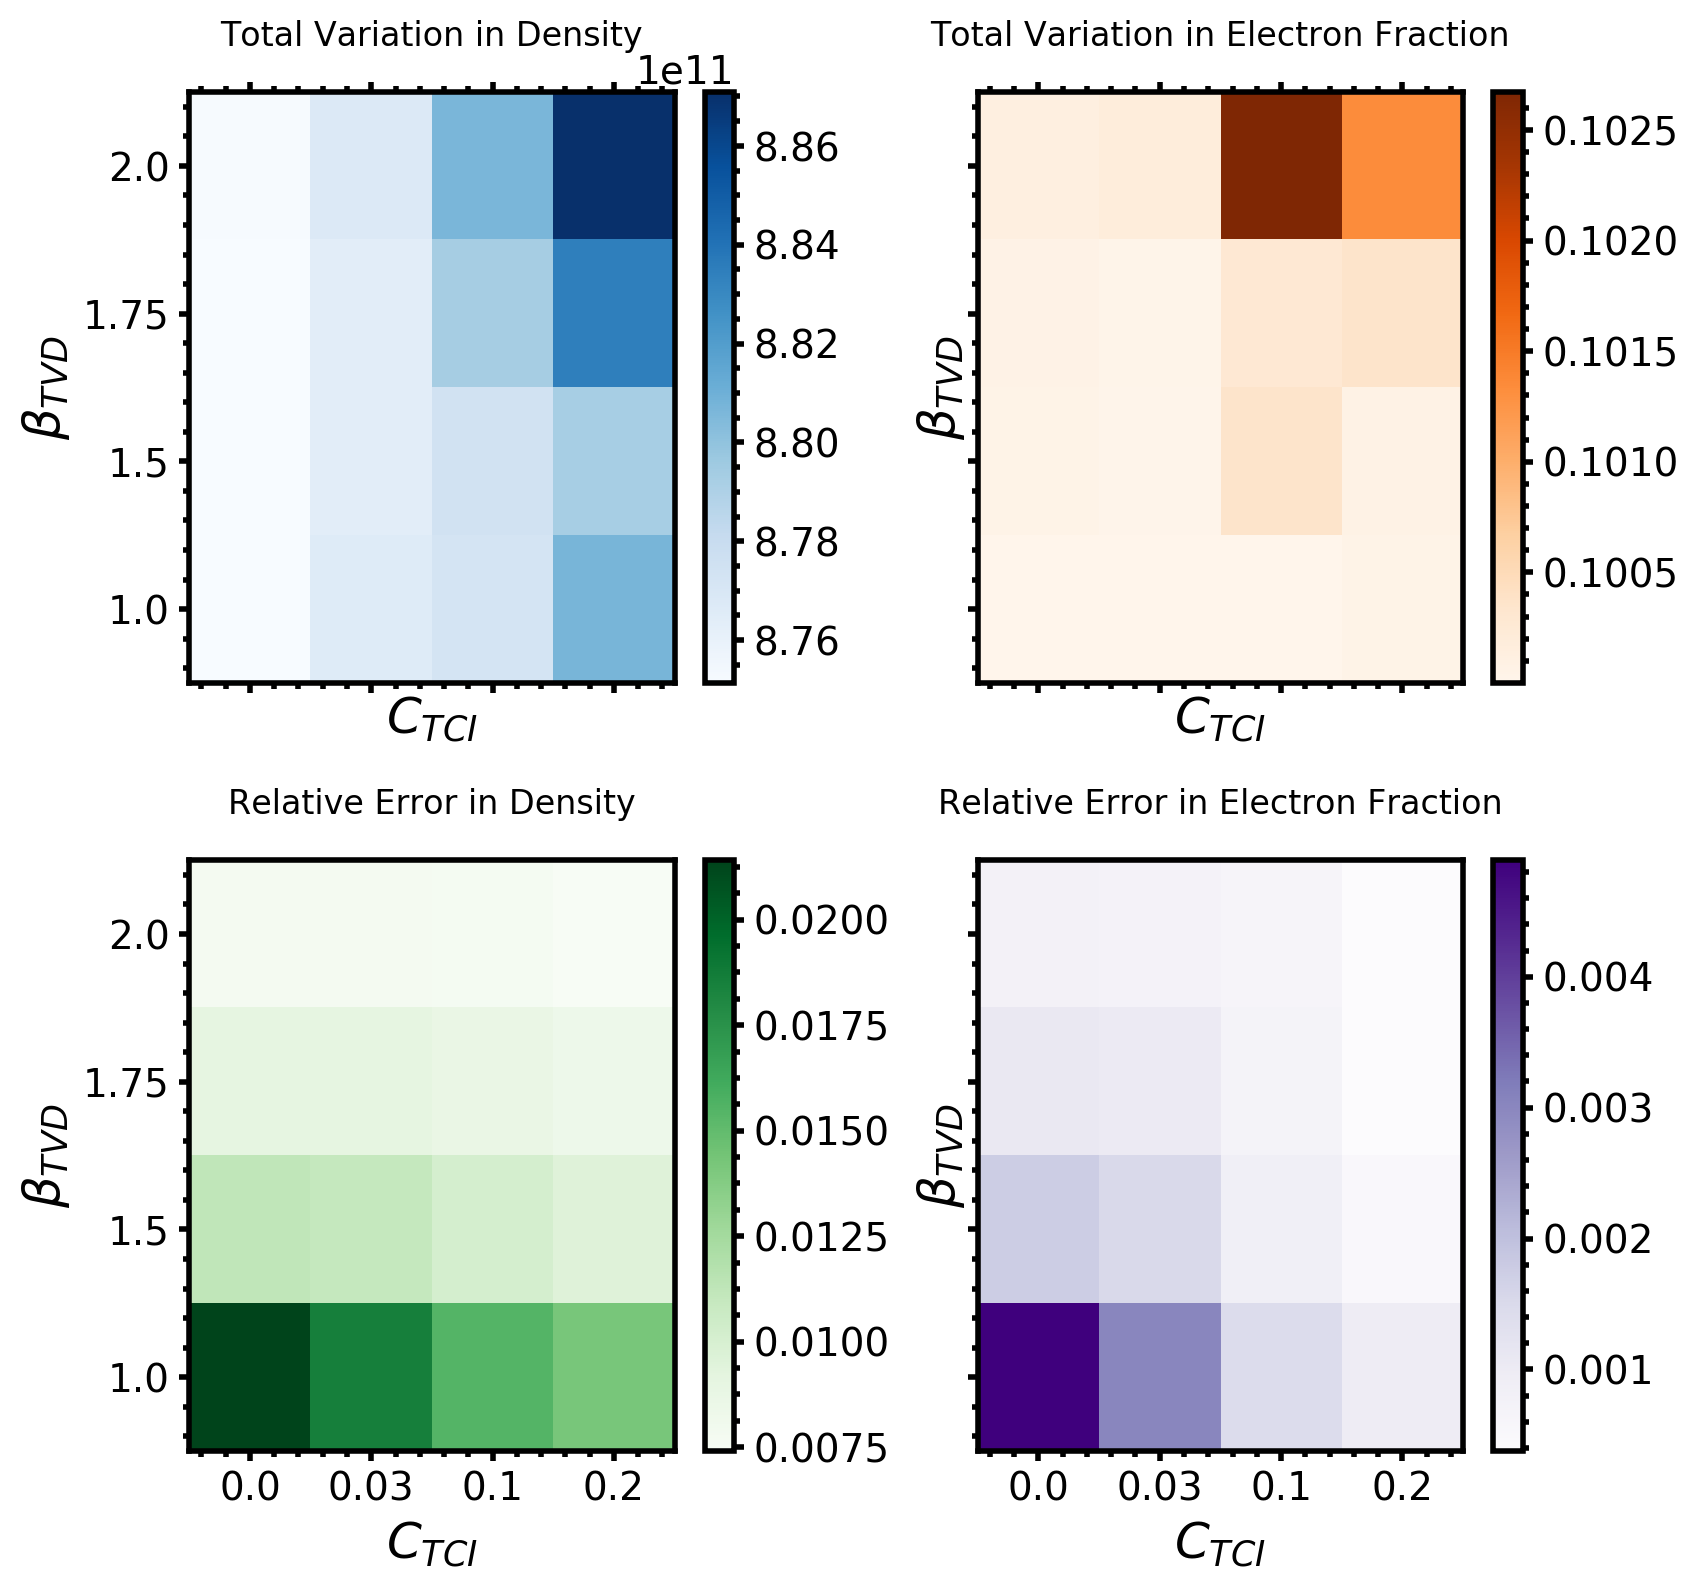
\includegraphics[width=32pc, height=32pc]{./figures/error_tv_landscape.png}
%   \caption{\label{fig:landscape} Error - total variation landscapes for various
%   values of the limiting parameters $C_{TCI}$ and $\beta_{TVD}$.}
% \end{figure}

\begin{figure}[h!]
  \centering
  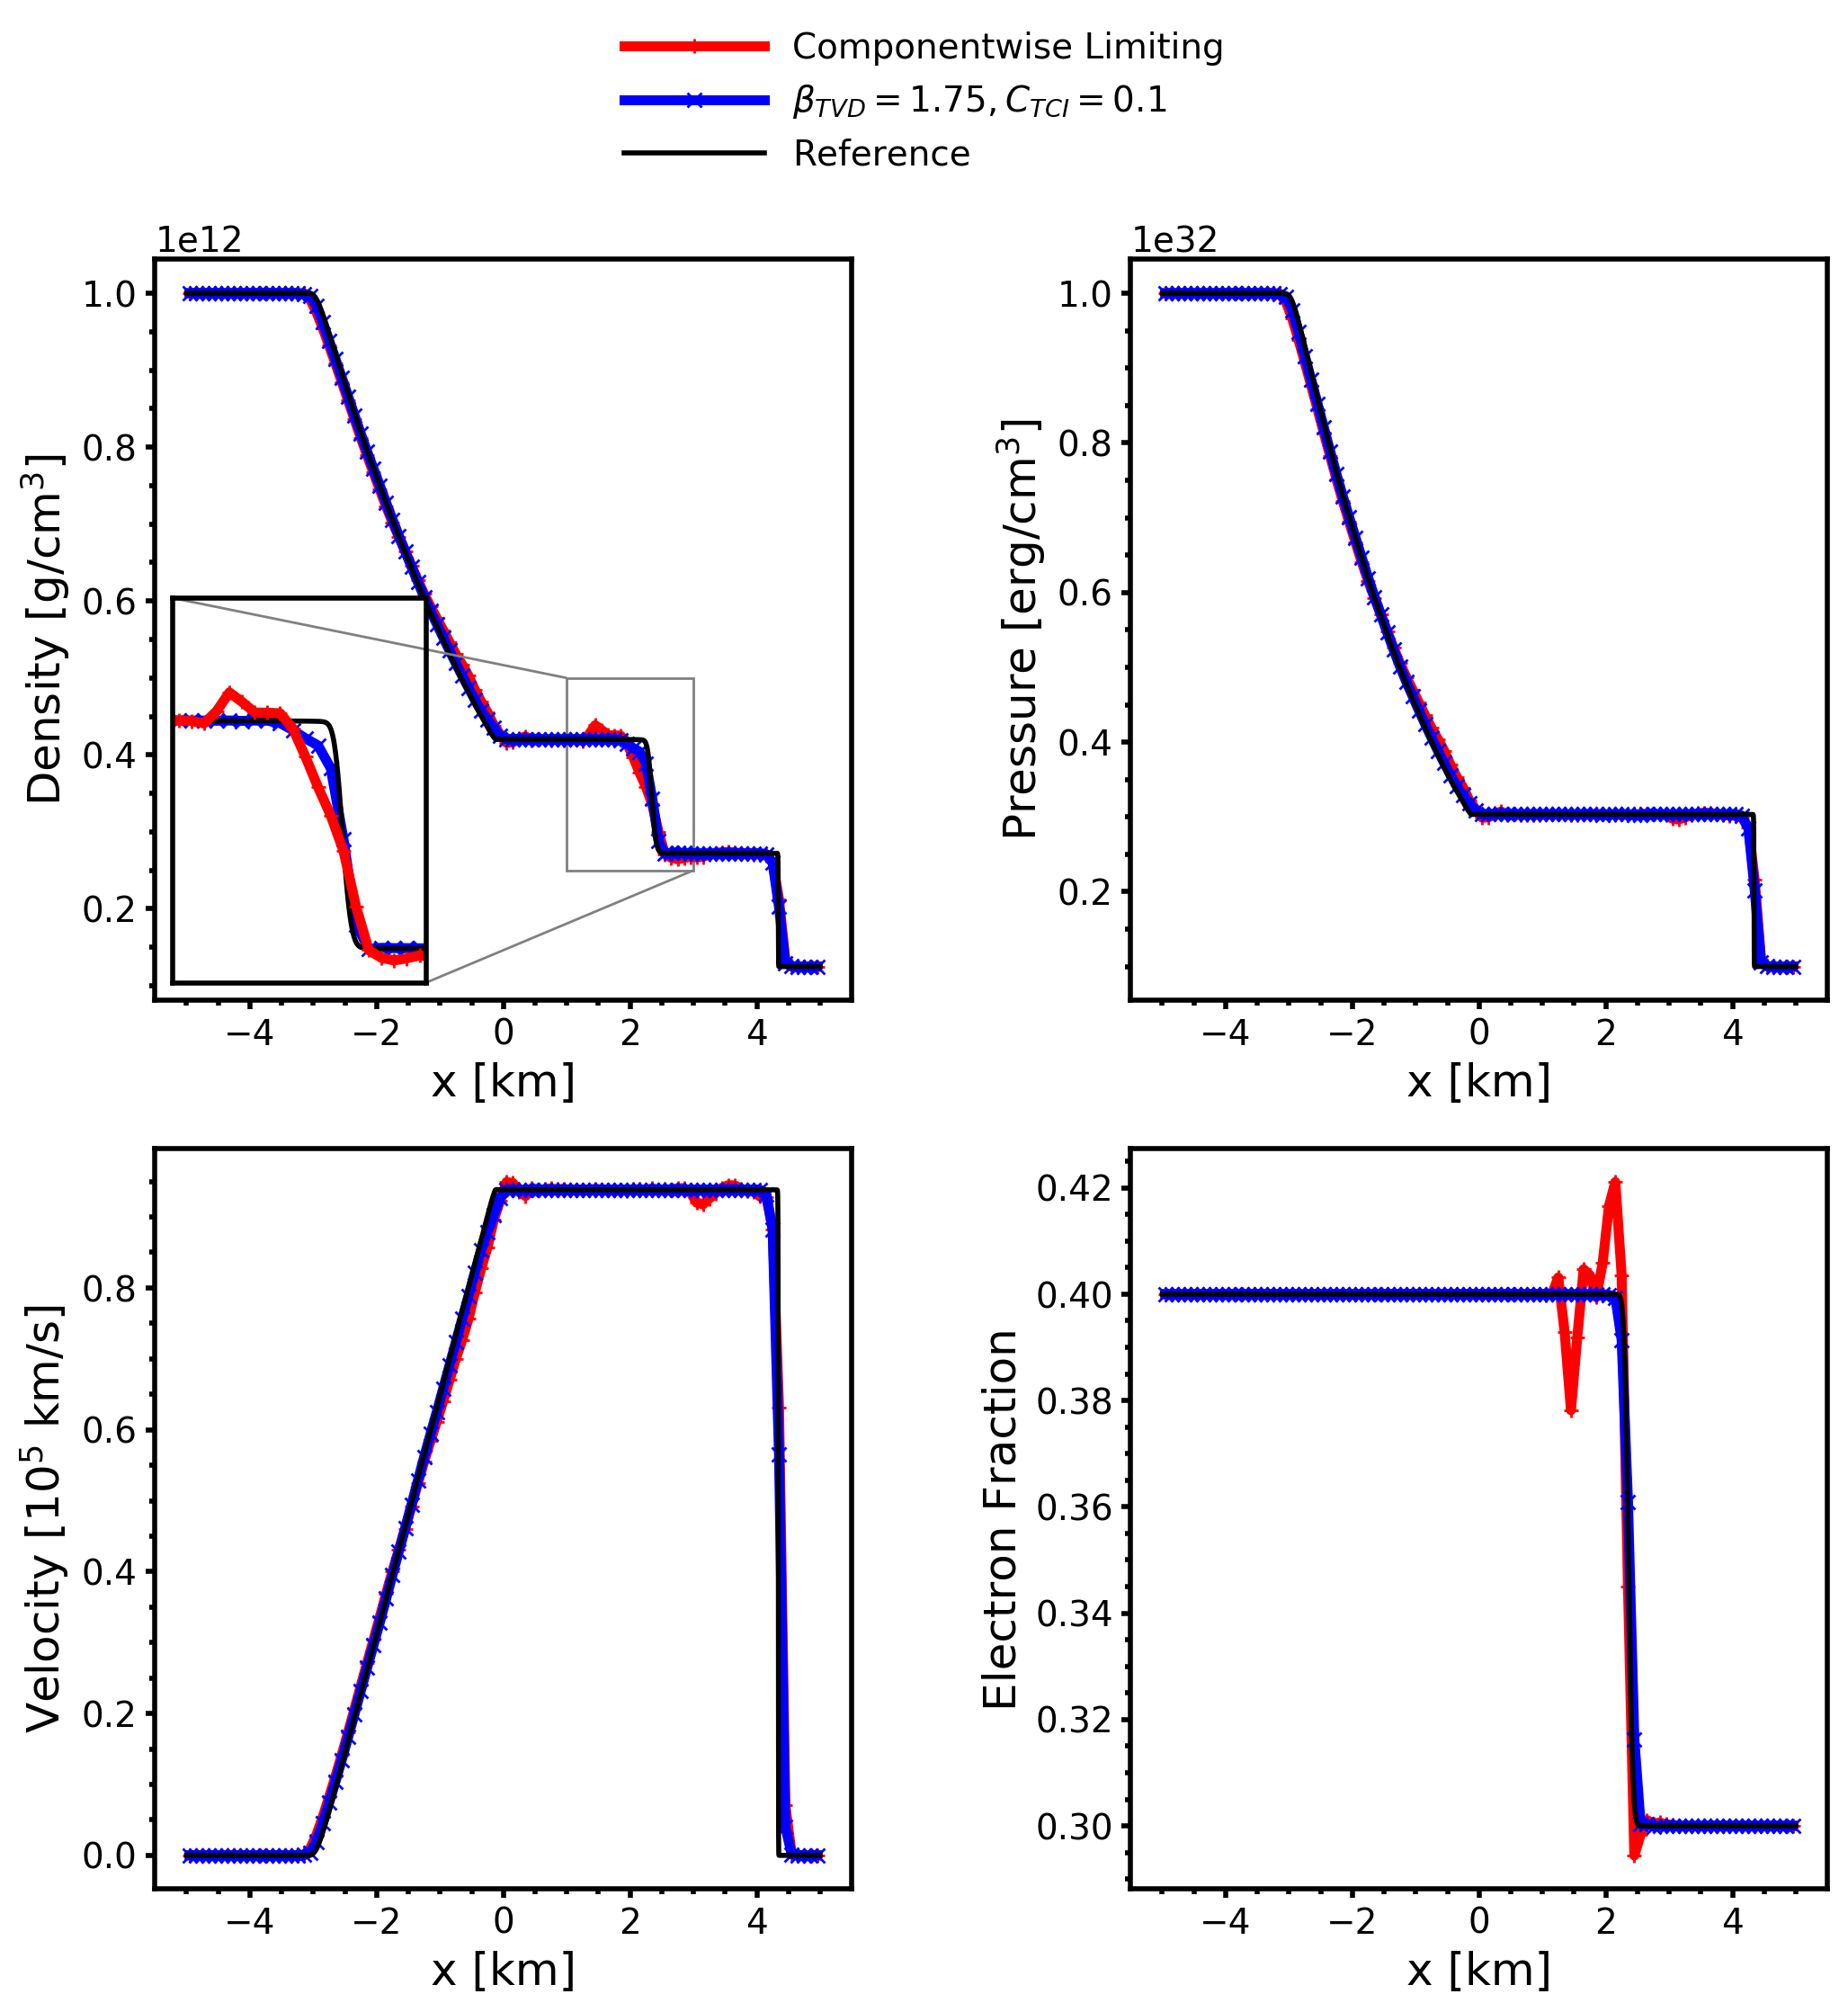
\includegraphics[width=36pc]{./figures/characteristic_cw.png}
  \caption{\label{fig:SodSedovCW} Numerical solution of Sod's problem using
  100 elements with characteristic limiting (blue) and componentwise limiting
  (red) compared with a reference solution using 10000 elements.}
\end{figure}

\subsection{High Density Regime}
This test is included to verify the performance improvements of the characteristic
limiting in a higher density regime. It is designed with the Sod problem in mind.
The computational domain is $D = [-5,5]$ km
with a discontinuity initially located at $x = 0$ km separating the left and right states

\begin{align}
  \mathbf{U}_{L} &= (10^{13}~\text{g~cm}^{-3}, 0\,, 3.712*10^{32}~\text{ergs~cm}^{-3}, 0.15*10^{12})^T\,\,\, \\
  \mathbf{U}_{R} &= (1.25*10^{12}~\text{g~cm}^{-3}, 0\, , 3.015*10^{31}~\text{ergs~cm}^{-3}, 0.169*10^{12})^T.
\end{align}

\noindent The test is run until $t = 0.05$ms with 100 elements
using $C_{\TCI} = 0.1$ and $\beta_{\TVD} = 1.2$. We chose a lower $\beta_{\TVD}$
here, as larger values resulted in internal energies outside of the
EOS table causing the test to fail, motivating the development of a
positivity limiter compatible with a tabulated nuclear matter EOS.
Inital state values were chosen to be consistent with
high-fidelity CCSN simulation code \chimera \citep{bruenn:2018} data.
Results are plotted in
Figure~\ref{fig:SodSedovHighDens}. Our method captures the main features
of the solution, but introduces more oscillations than in the lower density
case, even when using the characteristic limiter.
We notice an undershooting of the right side
of the contact discontinuity in the electron fraction not previously present
warranting further investigation.

\begin{figure}[h!]
  \centering
  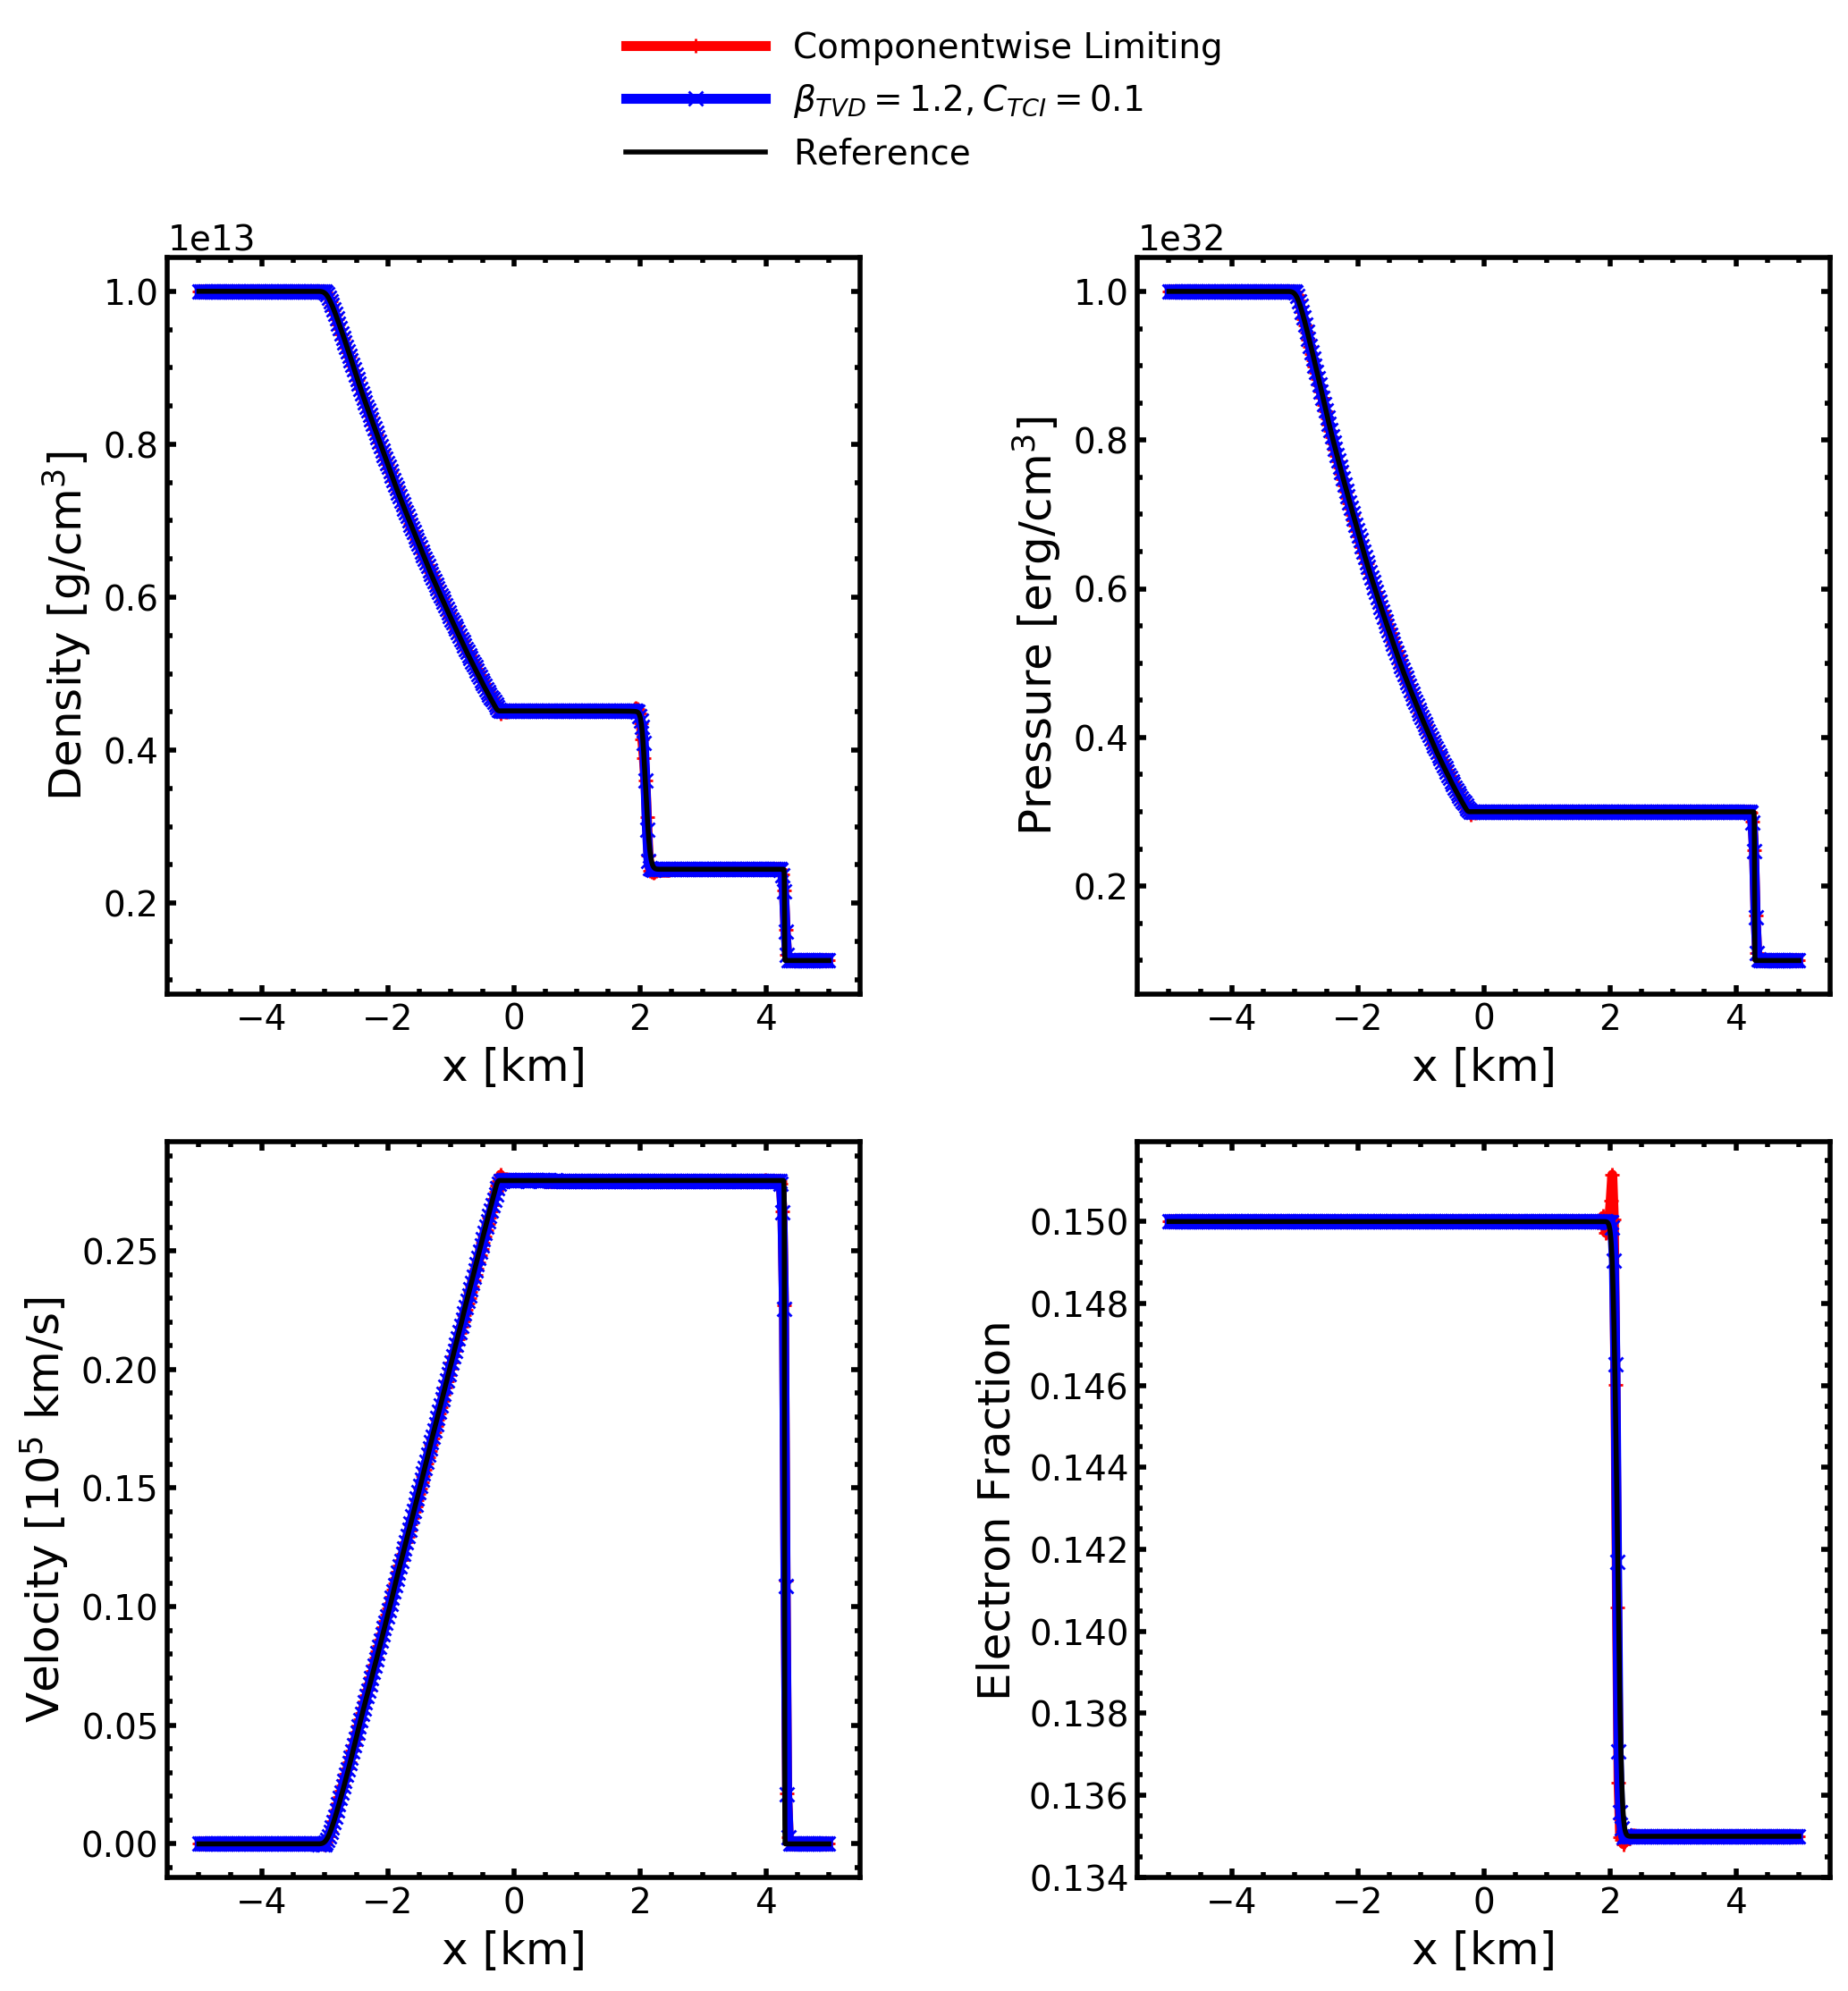
\includegraphics[width=36pc]{./figures/highDens.png}
  \caption{\label{fig:SodSedovHighDens} Results for the high density Sod-like problem
  computed using 100 elements and $C_{\TCI} = 0.1$ and $\beta_{\TVD} = 1.2$ at $t=0.05$ms.}
\end{figure}


\subsection{EOS Resolution Dependence}
\label{sec:eosRes}
In order to test the sensitivity of the limiter on the EOS table resolution,
we repeated the tests in Section~\ref{sec:optimal} with a higher resolution
SFHo EOS table. As before, tests are computed using 100 elements until
$t = 0.025$ms with characteristic limiting and the optimal limiting parameters determined in
Section~\ref{sec:param} and compared to a reference solution computed using
10000 elements. Results for both tables are plotted in Figure~\ref{fig:SodSedovSFHoRes}.
We find nearly no sensitivity to the table resolution, with the exception of
minor differences in density to the left of the contact discontinuity.
\begin{figure}[h!]
  \centering
  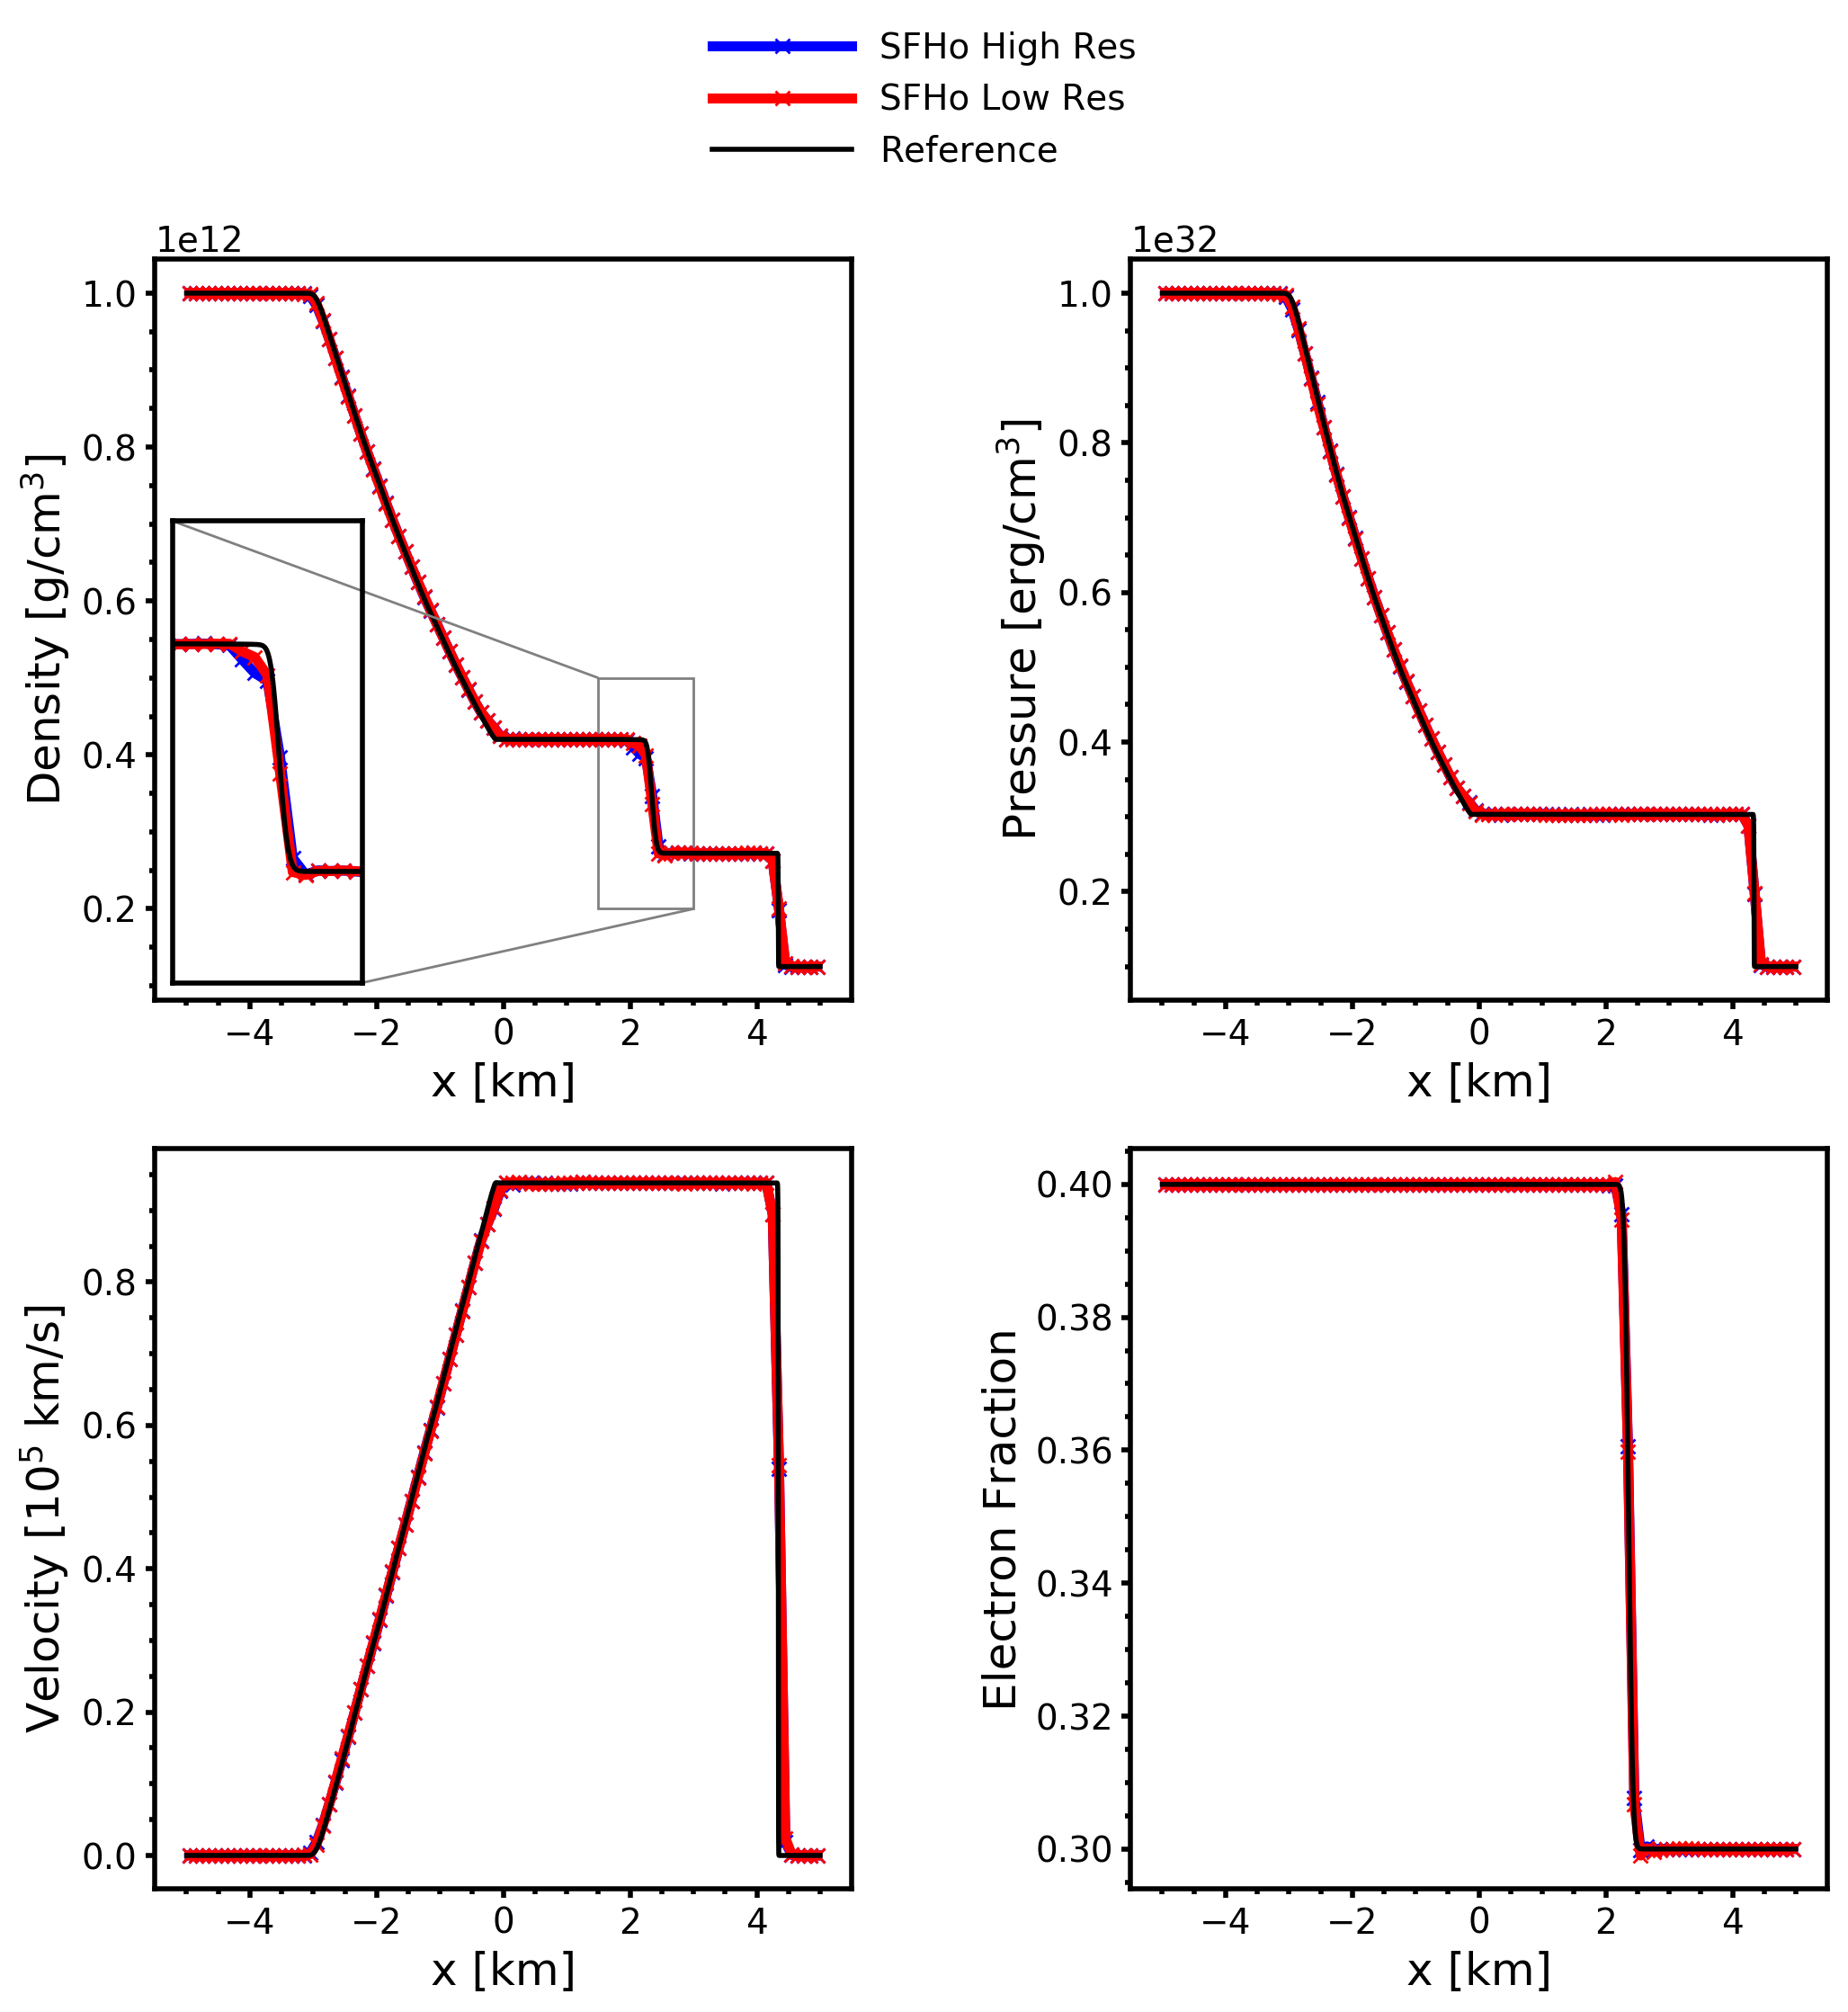
\includegraphics[width=36pc]{./figures/eos_res.png}
  \caption{\label{fig:SodSedovSFHoRes} Comparison of numerical solutions to
  Sod's problem using 100 elements with characteristic limiting and two
  different EOS table resolutions.}
\end{figure}


\subsection{EOS Table Sensitivity}
In order to probe the sensitivity of the method to the EOS table, we repeated
the tests conducted in Section~\ref{sec:optimal} using three different EOS tables:
the high resolution SFHo table from Section~\ref{sec:eosRes}, the SFHx table
(\textbf{citation}), and the DD2 table (\textbf{citation}).
As before, tests are computed using 100 elements until
$t = 0.025$ms with characteristic limiting and the optimal limiting parameters determined in
Section~\ref{sec:param}. We find nearly no sensitivity to the EOS table used in
the low density regime, with the exception of very small variations in density
to the left of the contact discontinuity. Future work includes testing the
sensitivity to the EOS table in higher density regimes.
\begin{figure}[h!]
  \centering
  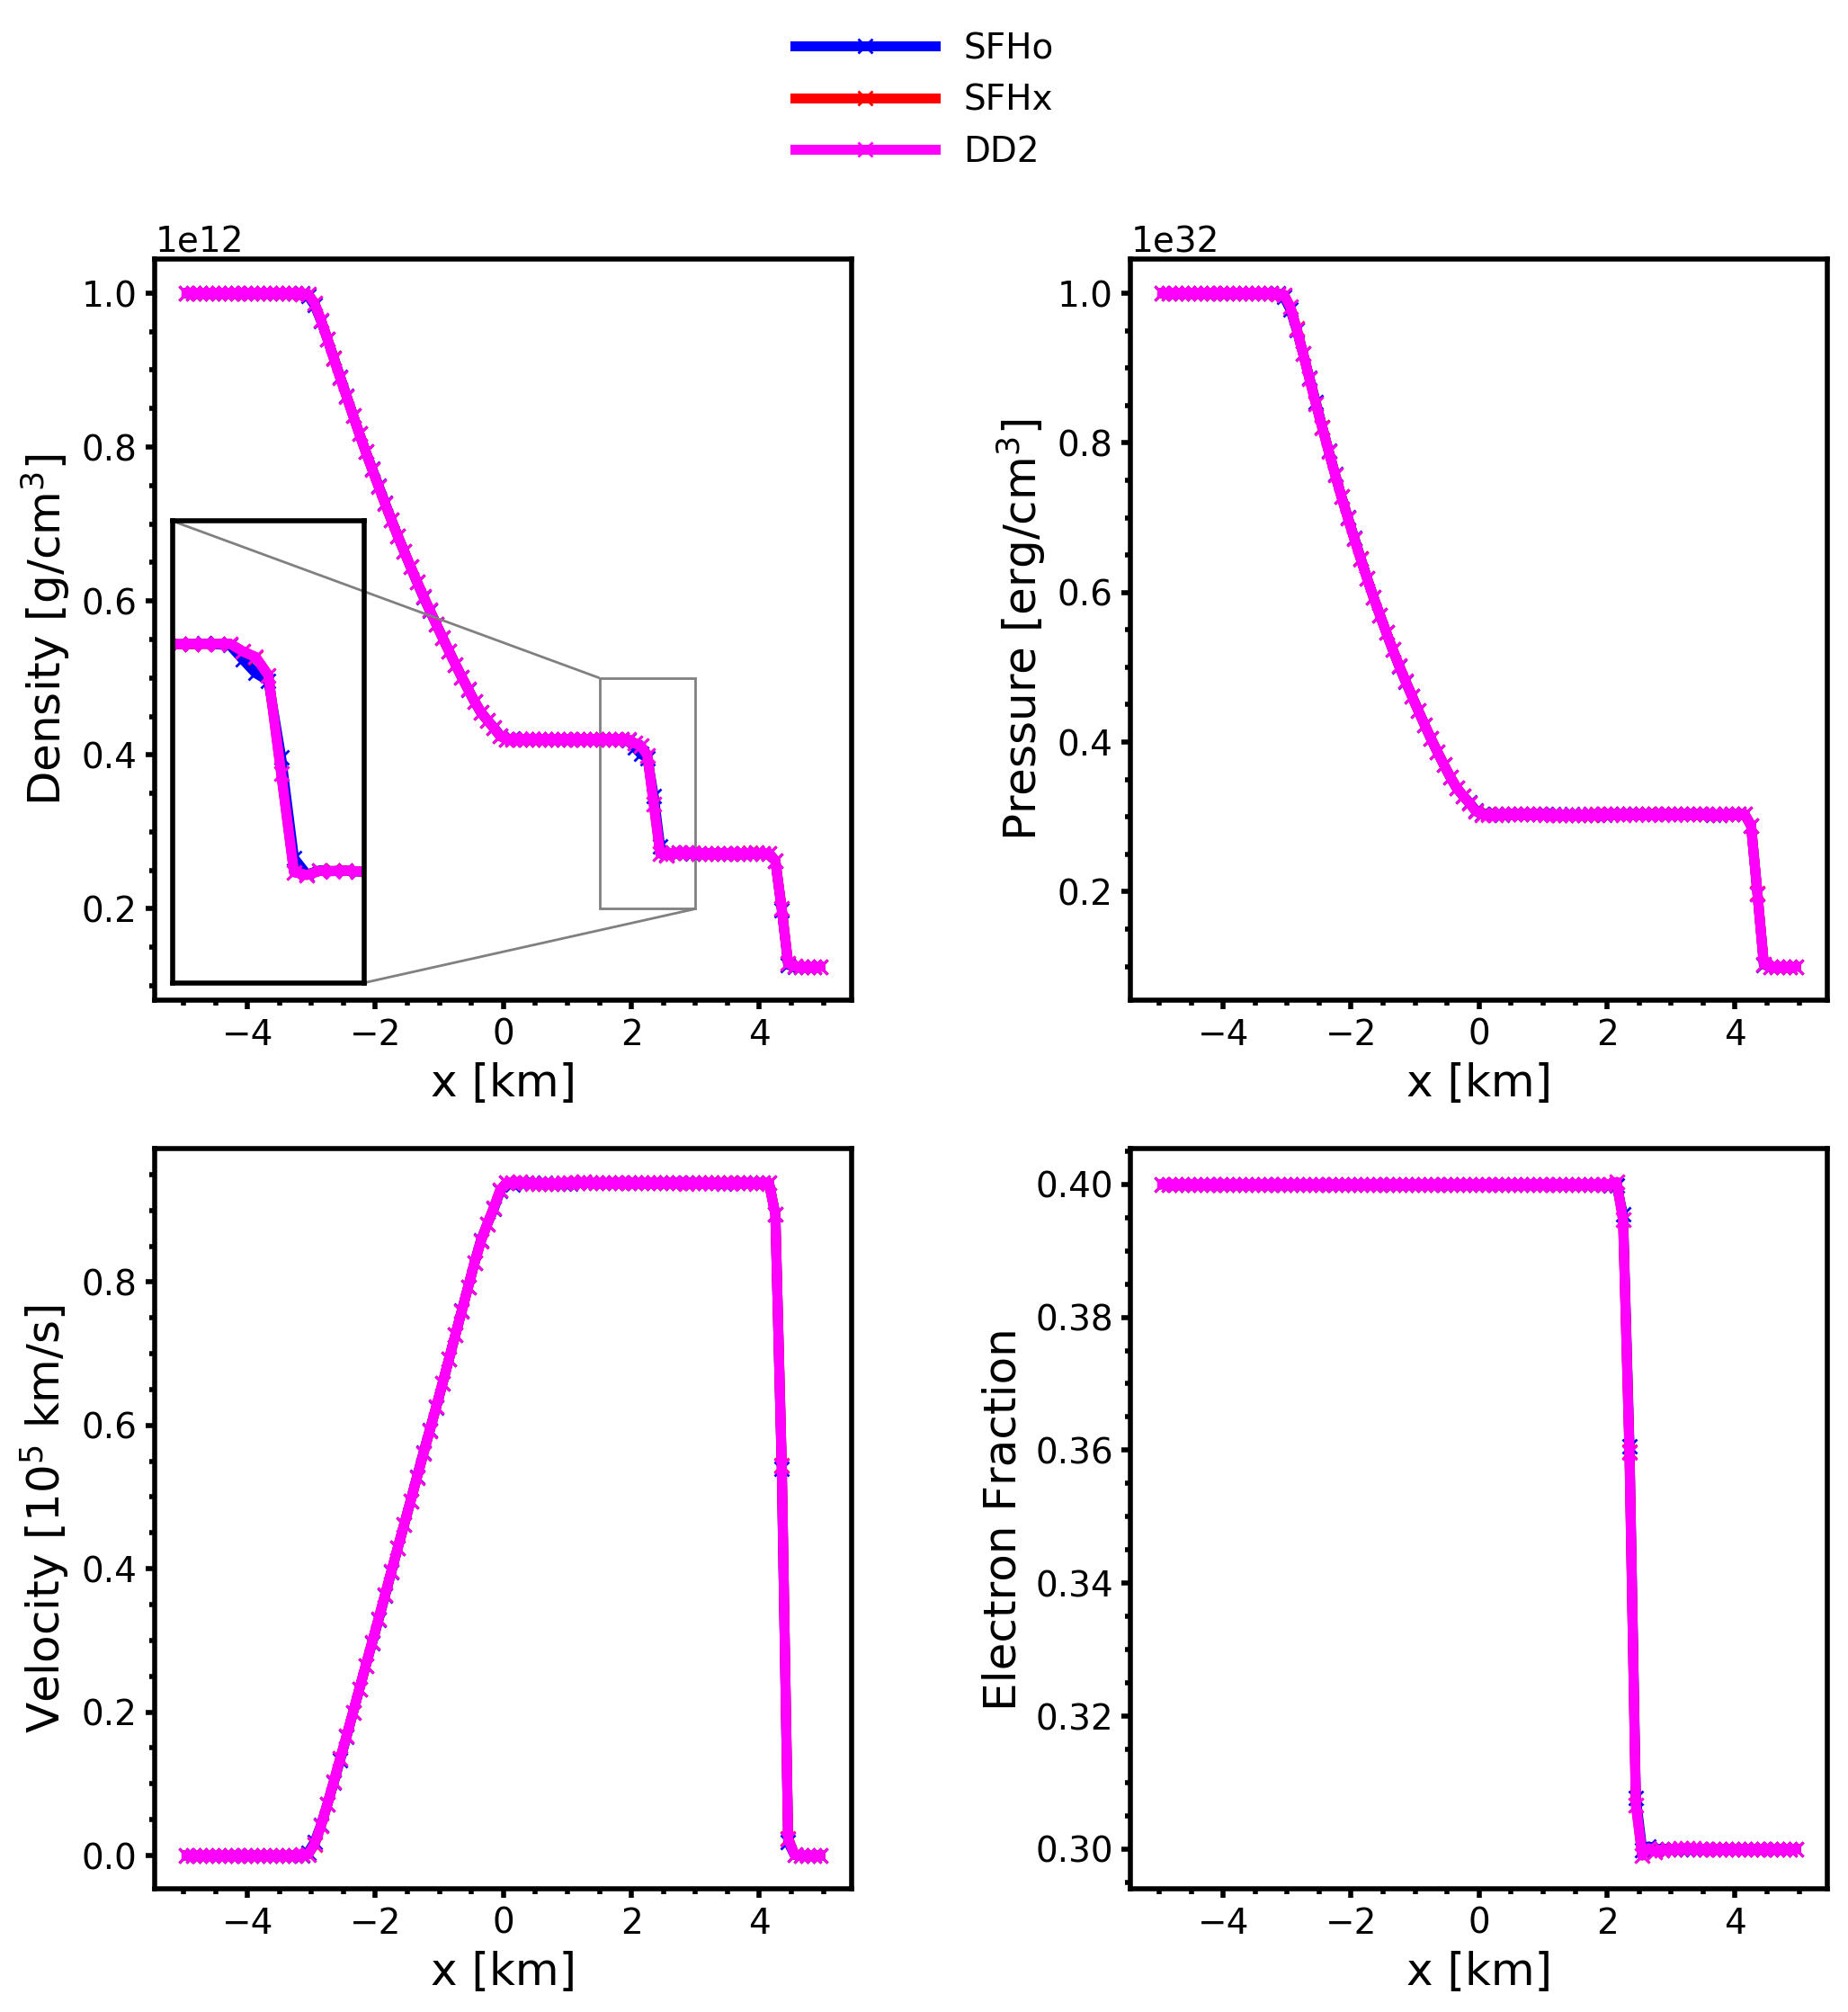
\includegraphics[width=36pc]{./figures/eos_all.png}
  \caption{\label{fig:SodSedovEOS} Comparison of numerical solutions to
  Sod's problem using 100 elements with characteristic limiting and three
  different EOS tables.}
\end{figure}
%\FloatBarrier

\section{Conclusions}

We have presented preliminary developments and numerical results for a
characteristic limiter to be used with solvers of the non-relativistic
Euler equations of gas dynamics in the {\bf t}oolkit for {\bf h}igh-{\bf or}der
{\bf n}eutrino-r{\bf ad}iation hydr{\bf o}dynamics (\thornado). The results
presented from a suite of 1D test problems, based around Sod's 1D shock
tube problem, demonstrate the performance of the characteristic limiter
compared to the componentwise limiter. Moreover, after performing a parameter
study on the limiter parameters, we found optimal limiting
parameters for use with the Sod problem. While the optimal limiting parameters
tend to be problem dependent, we hope to investigate if such an optimal
parameter exists for CCSN applications. Tests with various EOS tables and
table resolutions showed little to no sensitivity to the table or its
resolution in the tests studied. For future work, we will extend these studies
to other higher density regimes applicable to the CCSN environment.
Planned near-future work on the nuclear equation of state compatibility of
\thornado\, includes the development of a positivity limiter and extension of
the characteristic limtier to handle relativistic and curvilinear problems.

\acknowledgements
We thank people.

\software{
  \href{https://matplotlib.org/}{Matplotlib} \citep{hunter:2007a},
  \href{http://www.numpy.org/}{NumPy} \citep{walt:2011},
  \href{https://www.scipy.org/}{SciPy} \citep{jones:2001},
  }

\appendix

\section{Derivatives}
Derivatives of pressure with respect to $\tau$, $\epsilon$, and n. \\
\begin{footnotesize}
\begin{eqnarray}
	\frac{\partial{P}}{\partial{\epsilon}} &=& \left(\frac{\partial{\epsilon}}{\partial{T}}\right)^{-1}\left(\frac{\partial{P}}{\partial{T}}\right) \\
	\frac{\partial{P}}{\partial{n}} &=& \frac{m_B}{\rho} \left[ \frac{\partial{P}}{\partial{y_e}} -
          \frac{\partial{\epsilon}}{\partial{y_e}}\left(\frac{\partial{\epsilon}}{\partial{T}}\right)^{-1}\left(\frac{\partial{P}}{\partial{T}}\right)\right]\\
	\frac{\partial{P}}{\partial{\tau}} &=& -\tau^{-2} \left[ \frac{\partial{P}}{\partial{\rho}} - \frac{y_e}{\rho} \left( \frac{\partial{P}}{\partial{y_e}} -
          \frac{\partial{\epsilon}}{\partial{y_e}} \left(\frac{\partial{\epsilon}}{\partial{T}}\right)^{-1}\left(\frac{\partial{P}}{\partial{T}}\right)\right) -
          \frac{\partial{\epsilon}}{\partial{\rho}}\left(\frac{\partial{\epsilon}}{\partial{T}}\right)^{-1}\left(\frac{\partial{P}}{\partial{T}}\right)\right]
\end{eqnarray}
\end{footnotesize}




\bibliography{ms}


\end{document}
